%% Esempio per lo stile supsi
\documentclass[twoside]{supsistudent} 

\usepackage{listings}
\usepackage{pdflscape}
\usepackage{hyperref}
\usepackage[export]{adjustbox}
\usepackage{multicol}
% per settare noindent
\setlength{\parindent}{0pt}


\usepackage{color}

\definecolor{mygreen}{rgb}{0,0.6,0}
\definecolor{mygray}{rgb}{0.5,0.5,0.5}
\definecolor{mymauve}{rgb}{0.58,0,0.82}

\lstset{ 
  backgroundcolor=\color{white},   % choose the background color; you must add \usepackage{color} or \usepackage{xcolor}; should come as last argument
  basicstyle=\footnotesize,        % the size of the fonts that are used for the code
  breakatwhitespace=false,         % sets if automatic breaks should only happen at whitespace
  breaklines=true,                 % sets automatic line breaking
  captionpos=b,                    % sets the caption-position to bottom
  commentstyle=\color{mygreen},    % comment style
  deletekeywords={...},            % if you want to delete keywords from the given language
  escapeinside={\%*}{*)},          % if you want to add LaTeX within your code
  extendedchars=true,              % lets you use non-ASCII characters; for 8-bits encodings only, does not work with UTF-8
  frame=single,	                   % adds a frame around the code
  keepspaces=true,                 % keeps spaces in text, useful for keeping indentation of code (possibly needs columns=flexible)
  keywordstyle=\color{blue},       % keyword style
  language=C,                 % the language of the code
  morekeywords={*,...},            % if you want to add more keywords to the set
  numbers=left,                    % where to put the line-numbers; possible values are (none, left, right)
  numbersep=5pt,                   % how far the line-numbers are from the code
  numberstyle=\tiny\color{mygray}, % the style that is used for the line-numbers
  rulecolor=\color{black},         % if not set, the frame-color may be changed on line-breaks within not-black text (e.g. comments (green here))
  showspaces=false,                % show spaces everywhere adding particular underscores; it overrides 'showstringspaces'
  showstringspaces=false,          % underline spaces within strings only
  showtabs=false,                  % show tabs within strings adding particular underscores
  stepnumber=2,                    % the step between two line-numbers. If it's 1, each line will be numbered
  stringstyle=\color{mymauve},     % string literal style
  tabsize=2,	                   % sets default tabsize to 2 spaces
  title=\lstname                   % show the filename of files included with \lstinputlisting; also try caption instead of title
}



% Crea un capitolo senza numerazione che pero` appare nell'indice %
\newcommand{\problemchapter}[1]{%
  \chapter*{#1}%
  \addcontentsline{toc}{chapter}{#1}%
\markboth{#1}{#1}
}

% Numerazione delle appendici secondo norma
\addto\appendix{
\renewcommand{\thesection}{\Alph{chapter}.\arabic{section}}
\renewcommand{\thesubsection}{\thesection.\arabic{subsection}}}

% Crea una sezione senza numerazione che pero` appare nell'indice %
\newcommand{\problemsection}[1]{%
  \section*{#1}%
  \addcontentsline{toc}{section}{#1}%
\markboth{#1}{#1}
}

%----------------------------------------------------------------
%Definizione comandi
%----------------------------------------------------------------
\renewcommand{\contentsname}{Indice\vspace{5mm}}
\newcommand{\DecaTitolo}{Laboratorio - sviluppo applicazioni web}
\newcommand{\Decaa}{\newline\vspace{0.5mm}\newline\noindent}

\setcounter{secnumdepth}{5} 	%per avere più livelli nei titoli
\setcounter{tocdepth}{5}		%per avere più livelli nell'indice

\titolo{Progetto semestre: Libreria di supporto per riconoscimento immagini}
\studente{Andrea De Carlo \vspace{1em}\\ Roberto Trapletti }
\relatore{Giacomo Poretti}
\correlatore{}
\committente{DSwiss}
\corso{Ingegneria Informatica}
\modulo{M02042P}
\anno{2018/2019}

\begin{document}

\pagenumbering{alph}
\maketitle
\onehalfspacing
\frontmatter


\pagenumbering{roman}
\tableofcontents
% \listoffigures					% Opzionale
% \listoftables					% Opzionale


\problemchapter{Abstract} %rob
\problemsection{Abstract italiano}
Il progetto affronta come prima parte un problema di riconoscimento immagini utilizzando tecnologie mobile. L’obiettivo della libreria è quello di fornire le funzioni di supporto da utilizzare successivamente con un’applicazione di salvataggio password e documenti. Si vuole facilitarne il recupero permettendo all’utente di eseguire una ricerca tramite foto.
La seconda parte è un’analisi esplorativa delle tecnologie in ambito di Machine Learning utilizzabili a livello mobile. Per capire quali metodi sono usati attualmente e come funzionano, nella libreria è utilizzato un classificatore per aumentarne la robustezza, determinando se nell’immagine scattata dall’utente è presente uno schermo. 
\problemsection{Abstract inglese}
In the first part of this project, we deal with a problem of image recognition using mobile technologies. The purpose of this library is to provide the support functions to be used later with an application that saves passwords and documents. The goal is to facilitate recovery of the access keys by allowing the user to search through photos.
The second part of this research is an exploratory analysis of the technologies in Machine Learning that can be used on a mobile context. To apply an idea of understanding of methods that are currently used and how they work, we added a classifier in the library to increase its robustness, determining if a screen is present in the image taken by the user.


\problemchapter{Progetto assegnato} %rob
\problemsection{Descrizione}
Lo scopo del progetto è quello di rilevare tramite smartphone indirizzi (URL) o codici particolari testuali (per esempio password) visualizzati su uno schermo, per esempio di un PC.

Si tratta quindi di realizzare un programma per smartphone Android che tramite funzioni di Computer Vision sia in grado di riconoscere dei caratteri (OCR) in determinate zone dello schermo.

Il progetto è realizzato su richiesta della ditta DSwiss che fornirà dettagli supplementari e seguirà il progetto per requisiti e verifiche dei risultati ottenuti.

\problemsection{Compiti}
\begin{itemize}
\item Sviluppare un'applicazione Android
\item Riconoscere uno schermo
\item Estrarre i caratteri visualizzati sullo schermo
\item Isolare URL da indirizzi o codici esposti in zona precisa schermo
\end{itemize}

\problemsection{Tecnologie}
Java, Android, OpenCV per Android o altri framework particolari di OCR disposnibili per Android

\newpage
\mainmatter
\pagenumbering{arabic}
\setcounter{page}{1}



\chapter{Introduzione}
\section{Contesto del progetto}
    %dire che per la ditta è importante un concetto di intelligenza artificiale
    La ditta committente DSwiss dispone di una applicazione sia pc client che mobile di gestione delle password. Nello stato attuale, queste password vengono salvate all'interno di un DB locale sempre a disposizione dell'utente.
    \Decaa
    Hanno pensato di aggiungere una nuova caratteristica, ovvero un sistema di ricerca automatica della password da inserire, tramite una fotografia della pagina di login.
    Vorrebbero quindi applicare delle tecnologie (computer vision) per comprendere da una immagine appena scattata, il dominio della pagina web (sito) e recuperarne la password associata.
    \Decaa
    In un secondo momento, dopo lo svolgimento dell'obbiettivo prefissato,
    la ditta in questione ha suscitato dell'interesse importante per il concetto di intelligenza artificiale. Come obbiettivo aggiuntivo, siamo andati quindi ad eseguire una analisi esplorativa dei concetti base di machine learning in ambito PC e mobile.
    
\section{Evoluzione e adattamento degli obbiettivi}
\subsection{Preambolo}
\subsection{Obbiettivi iniziali della richiesta}
Durante l’assegnazione dei lavori di semestre, per questo progetto erano stati prefissati i seguenti obbiettivi:

\begin{itemize}
\item Sviluppare un'applicazione Android
\item Riconoscere uno schermo
\item Estrarre i caratteri visualizzati sullo schermo
\item Isolare URL da indirizzi o codici esposti in zona precisa schermo

\end{itemize}

Durante un primo incontro con il committente, abbiamo scoperto che questi obbiettivi non erano confacenti alla effettiva richiesta esposta dalla ditta. Abbiamo pertanto stilato, con l’aiuto del relatore e del committente, una nuova lista degli obbiettivi.

% METTERE GLI OBBIETTIVI NUOVI IN MANIERA POLITICALLY CORRECT
\begin{itemize}
\item Ritornare un'informazione associata data una fotografia, (come il nome del sito)
\item Sviluppare una libreria per pc e/o android
\item Tutto quanto è da implementare in un contesto locale, senza l'ausilio di servizi in cloud o di un qualsiasi tipo di dispositivo in rete.
\end{itemize}

\subsection{Obbiettivi aggiuntivi alla richiesta iniziale}
Dato che il raggiungimento dell'obbiettivo di recuperare il nome del sito da una foto scattata con il telefono è stato eseguito con buone tempistiche (lato desktop), il committente ha mostrato il suo interesse nell'approfondire altre tematiche, in particolare machine learning in ambito mobile.
\Decaa
È stato quindi deciso di approfondire questa tematica, tramite una analisi esplorativa con uno studio di fattibilità in ambito di machine learning su smartphone (computazione locale) senza ausilio di servizi esterni, come server remoti o servizi online. 
\Decaa
Pertanto l'obbiettivo aggiuntivo è quello di implementare una piccola funzionalità che sfrutti le tecnologie di machine learning all'interno della nostra libreria.

\chapter{Requisiti e specifiche} 
Il requisito più importante e limitante a livello di programmazione è quello che tutta la libreria deve utilizzare solo ed unicamente le risorse locali dei dispositivi mobile, per questioni di sicurezza. Questo significa che i servizi come le API Vision di Google \cite{googleVision}, le API Computer Vision di Azure della Microsoft \cite{microsoftAzure}o Amazon Rekognition di Amazon \cite{amazonReko}, non sono utilizzabili. 
\Decaa
La ditta DSwiss utilizza Xamarin come soluzione per lo sviluppo della loro applicazione. Per questo motivo la libreria sarà implementata e testata utilizzando lo stesso strumento.

\chapter{Fase analitica}
\section{Stato dell'arte} %rob
\subsection{Feature detection}%rob
Quando giochiamo con i puzzle, il nostro cervello esegue due operazioni significative: determina quali punti di un singolo pezzo sono importanti, che quindi possano essere comparati facilmente, e cerca di descriverli, in modo da trovare collegamenti con gli altri pezzi. In computer vision eseguire una feature detection significa ricercare quali punti possono essere utilizzati per una comparazione. Esistono diversi algoritmi che si possono basare su: \begin{itemize}
\item Contorni, bordi
\item Angoli
\item Regioni
\item Creste
\end{itemize}
Una volta trovati questi punti bisogna anche trovare il modo più efficiente per descriverli. Per questo motivo esistono altri tipi di algoritmi chiamati "algoritmi di feature description".
Una volta ottenute i punti d'interesse e la loro descrizione, si possono cercare le stesse feature in altre immagini e quindi determinare la presenza di corrispondenze. 
Gli algoritmi più conosciuti sono:
\begin{itemize}
\item SIFT
\item SURF
\item BRIEF
\item KAZE
\end{itemize}
La libreria più utilizzata in questo ambito è OpenCV \cite{openCv}. È una libreria sotto 3-clause BSD License. Esiste il supporto per Python, Java e C++ e anche qualche binding di terze parti. Contiene delle implementazioni ottimizzate per la maggior parte dei comuni algoritmi e tecniche utilizzate in computer vision.
L'algoritmo che abbiamo potuto testare più performante è senz'altro il SURF\cite{surf}. Purtroppo è un algoritmo patentato e l'utilizzo ne richiede quindi una licenza apposita. Nei nostri progetti di test mobile abbiamo utilizzato il KAZE\cite{kaze} che richiede un po' più di tempo.
\subsubsection{Feature detection su smartphone}%rob
La libreria OpenCV ha un porting per Android e anche per IOS. Per lo sviluppo con strumenti pensati per il multiplatform, come Xamarin\cite{xamarin}, esistono delle librerie di terze parti. La ditta DSwiss utilizza come strumento di sviluppo proprio Xamarin, per questo motivo abbiamo cercato librerie disponibili in quest'ambito. Abbiamo scoperto Accord.NET\cite{accordNet}, che in teoria offre funzionalità di Machine Learning, di image processing, di computer vision e molto altro. Ha una versione leggera pensata per i dispositivi mobili. Altro punto positivo è la licenza: GNU Lesser Public License v2.1. Purtroppo, abbiamo provato a utilizzarla senza successo, dato che gli sviluppatori sono ancora ad una versione alpha e il build non funziona in determinate condizioni. Per questo motivo nella nostra libreria abbiamo utilizzato EMGU.CV\cite{emguCv}. È un wrapper .NET di OpenCV. Dispone di due modelli di licenza, una open source (GNU GPL license v3) o commerciale. Alcune funzionalità sono disponibili solo utilizzando la licenza commerciale. A scopo di test e didattico abbiamo chiesto e ricevuto una versione di prova della libreria completa. 
\subsection{Machine learning}%rob
\begin{quote}
    «Si dice che un programma apprende dall’esperienza \textbf{E} con riferimento a alcune classi di compiti \textbf{T} e con misurazione della performance \textbf{P}, se le sue performance nel compito \textbf{T}, come misurato da \textbf{P}, migliorano con l’esperienza \textbf{E}».
\end{quote}
    In pratica le tecniche di Machine Learning (ML) permettono ai computer di imparare dall'esperienza. ML si può suddividere in tre principali categorie: l'apprendimento supervisionato, l'apprendimento non supervisionato e l'apprendimento per rinforzo. La scelta del tipo di apprendimento da utilizzare dipende naturalmente dal problema da risolvere e dalla capacità computazionale del dispositivo che utilizzeremo.
    L'apprendimento supervisionato consiste nel fornire ad un sistema un dataset (raccolta di dati strutturata) di informazioni in input e il releativo risultato. Per affrontare il suo compito il computer analizza il dataset e cerca di trovare delle regole in base a quanto già visto. La risposta che fornirà sarà quella più probabile secondo le sue esperienze, quindi secondo i dati passati in ingresso. 
    L'addestramento non supervisionato differisce da quello supervisionato perché le informazioni che inseriamo all'inizio non sono classificate, i risultati non esistono. Il computer stesso deve definire le caratteristiche di una classe. Viene utilizzato in problemi di clustering, cioè il raggruppare in diversi insiemi determinati elementi.
    L'apprendimento per rinforzo è utilizzato in ambienti dinamici dove il computer deve raggiungere un obbiettivo. Si utilizza un sistema di ricompense e penalità. L'esempio più comune è l'utilizzo nelle auto senza pilota. 
    
    \subsubsection{Deep learning e Neural network}
    Nella nostra libreria utilizzeremo il deep learning per renderla più robusta e per determinare se ci sono e quali loghi in una determinata immagine. Il deep learning è una sotto categoria del machine learning e consiste nel produrre modelli di apprendimento su più livelli. 
    In generale, apprende nuove nozioni da ciò che impara nei livelli precedenti. Pensate ad un'immagine di un gatto. Dopo una prima analisi dell'immagine determina che ci sono, occhi, baffi, pelo, ecc... Al prossimo livello, grazie alle informazioni raccolte in precedenza capisce che si tratta di un gatto. Potremmo anche aggiungere un ulteriore livello di consapevolezza e capire di quale razza si tratta. Il deep learning come tale, ha fatto grandi passi negli ultimi anni, grazie anche alla reperibilità sempre maggiore di dataset di ogni tipo. Al centro del deep learning si trovano le neural network. Le reti neurali sono principalmente dei modelli matematici, che permettono di produrre una risposta in uscita dato un determinato input.
Queste tipologie di modelli matematici sono composti da livelli di "neuroni" stratificati, ovvero dei componenti procedurali (di calcolo o statistica) che simulano lo stesso funzionamento di un neurone (nodo) e le relative sinapsi (collegamento tra nodi). Questi strati si suddividono in strati di input, strati nascosti e strato finale, come da immagine.

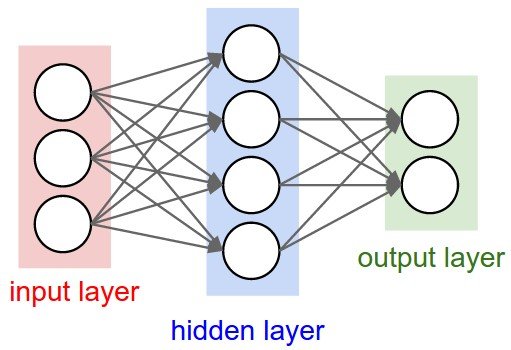
\includegraphics[width=\textwidth]{Pictures/neural_net.jpeg}

\subsubsection{Machine learning su smartphone}%rob
L'utilizzo del Machine Learning sui dispositivi mobili non è complicato. La parte che richiede più risorse computazionali infatti è la fase di training di un modello. Una volta ottenuto questo modello possiamo caricarlo nella nostra applicazione e utilizzarlo. I framework a disposizione sono molti, ma abbiamo avuto modo di testarne qualcuno come "ML .NET"\cite{mlNet} che però sono risultati ancora non utilizzabili in termini di preparazione dell'ambiente di sviluppo e in termini di prestazioni. Tuttavia sono in fase di forte sviluppo, quindi ci aspettiamo un netto miglioramento di questo framework durante i prossimi mesi. Per la nostra libreria e i nostri test, abbiamo provato quindi a utilizzare Tensorflow\cite{tensorFlow}. Il test è avvenuto con successo sulla versione desktop mentre i binding della libreria presenti in Xamarin non funzionavano. Tensorflow però sta sviluppando un'alternativa per i dispositivi mobile chiamata Tensorflow Lite. Non abbiamo avuto modo di testarlo, ma quello che abbiamo capito è che è meglio scrivere codice nativo senza passare da soluzioni multipiattaforma. Librerie cross-platfrom per Machine Learning e Computer Vision sono ancora in uno stato troppo acerbo. 

\subsubsection{Dataset e modelli}%rob
Per il nostro progetto e per poter testare gli strumenti in ambito di Machine Learning, abbiamo cercato di risolvere un problema di image recognition. Vogliamo verificare che in un'immagine sia presente o meno un monitor, uno schermo. Il primo passo per affrontare questo problema è trovare tante foto di monitor o schermi. In un primo momento abbiamo quindi optato per riaddestrare l'ultimo layer di una neural network già pronta. 
Per trovare molte immagini di monitor abbiamo utilizzato uno script python di un progetto git pubblico\cite{googleDown} "google-images-download". Grazie a questo script si può eseguire il download di tot immagini da una ricerca in Google Immagini, specificandone anche il formato, la dimensione, ecc... Dopo aver scaricato le immagini le abbiamo processate per ridimensionarle tutte a 224x224 pixel. Questo perché addestrare l'ultimo layer di una neural network con immagini di dimensioni maggiori richiede più risorse e quindi di più tempo. Lo script è molto semplice:
\begin{lstlisting}[language=Python]
from PIL import Image
import os
import sys

directory = sys.argv[1]
saveDirectory = sys.argv[2]

for file_name in os.listdir(directory):
  print("Processing %s" % file_name)
  image = Image.open(os.path.join(directory, file_name))

  x,y = image.size
  new_dimensions = (224, 224)
  output = image.resize(new_dimensions, Image.ANTIALIAS)

  output_file_name = os.path.join(saveDirectory, file_name)
  output.save(output_file_name, "JPEG", quality = 95)

print("All done")
\end{lstlisting}

Tuttavia, dopo ulteriori ricerche, abbiamo recuperato un modello pre-addestrato per il riconoscimento di immagini tra cui l'etichetta monitor o screen è presente nei nodi di output. Si chiama MobileNet\cite{mobileNet} ed è opensource. Si possono trovare differenti modelli (basati sullo stesso dataset ma addestrati in modo diverso) che differiscono per prestazioni, dimensioni e precisione.

\section{Studio delle soluzioni - obiettivi iniziali}
Tenendo in considerazione gli obbiettivi iniziali di questo progetto, siamo andati a cercare una possibile soluzione per la richiesta commissionata.
\Decaa
L'obbiettivo principale di questa richiesta è quello di ricavare una associazione tra: foto appena scattata di una schermata di login -> corrispettiva informazione (ad esempio il nome di dominio di una pagina web)
Per risolvere questa richiesta, sono disponibili svariate soluzioni, con diverse tecnologie di appoggio, per esempio:
\begin{itemize}
\item Tecnologie di optical character recognition (OCR)
\item Tecnologie di computer vision per feature detection e feature matching
\end{itemize}
È stato quindi necessario coinvolgere il committente per identificare su quale tecnologia erano interessati. Ci hanno indicato di analizzare delle possibili soluzioni basate su computer vision. In questo modo la libreria può funzionare anche con schermate di login che sfruttano servizi esterni di autenticazione (OAuth).

\subsection{Accord.NET e Xamarin}

\includegraphics[width=0.5\textwidth]{Pictures/accord_net.png}
\newline
Accord.NET è un framework in .NET per machine learning, data processing, Image processing, computer vision e molto altro. Dispone ulteriormente di un lightweight framework adattato per lo sviluppo su mobile.
\Decaa
Distribuita sotto licenza GNU Lesser Public License v2.1
\Decaa
Purtroppo, durante una fase di test, abbiamo riscontrato parecchi problemi di integrazione. La causa è data dal fatto che questa libreria si trova in uno stato di test, in versione alpha e con delle problematiche di build in determinate condizioni.
\Decaa
Sebbene questo progetto sia in continua evoluzione, abbiamo deciso di scartarlo.

\subsection{ML.NET e Xamarin}
ML.NET è un framework per machine learning fornito da Microsoft, open source e multipiattaforma.
Fornisce delle automazioni per la gestione dei dataset (raccolta di dati) ed il successivo trattamento, come l'estrapolazione delle caratteristiche e la costruizione di classificatori.
\Decaa
Questa libreria sta puntando sulla produzione di codice utilizzabile su dispositivi mobili, con la possibilità di integrazione di altre librerie come "Tensorflow", "Accord.net" e altre. Per questo motivo ha suscitato il nostro interesse.
\Decaa
Con una successiva ricerca, abbiamo scoperto che ML.NET per ora non dispone delle caratteristiche necessarie per risolvere la richiesta commissionata. Infatti, non fornisce delle funzionalità per processo di immagine.
\Decaa
Abbiamo deciso di scartare anche questo framework.

\subsection{EmguCV e Xamarin}

\includegraphics[width=0.5\textwidth]{Pictures/emgu.jpeg}
\newline
Emgu è una libreria wrapper che permette di eseguire il framework opencv su .net facendo quindi da interfaccia logica di traduzione tra i due.
\Decaa
OpenCV è un framework molto conosciuto per il processo di immagini, infatti esso è supportato da una grande comunità di sviluppatori. Nell'ambito del nostro incarico da svolgere, OpenCV fornisce tutte le funzionalità necessarie per il processo di immagine.
\Decaa
A livello di costo, EmguCV dispone di due licenze:
\begin{itemize}
\item Licenza open source ma con libreria limitata (priva della versione mobile)
\item licenza commerciale: 400 dollari per 1 licenza sviluppatore, 800 dollari fino a 25 sviluppatori
\end{itemize}
Per fini didattici, Emgu ci ha fornito una versione demo della libreria commerciale, comunque limitata ma con la possibilità di porting su mobile.

\subsection{Decisione soluzione}
Per lo svolgimento della richiesta iniziale, abbiamo deciso in collaborazione con il committente, di utilizzare la soluzione composta da EmguCV e Xamarin come ambiente di sviluppo. Determinante è stata la notorietà di OpenCV con le sue funzionalità conosciute ed il suo supporto dato dalla community.

\section{Studio delle soluzioni - obiettivi aggiuntivi}
Tenendo conto degli interessi suscitati dal committente, effettuiamo una ricerca sulle possibili soluzioni presenti attualmente nell'ambito di machine learning su dispositivi mobili.
\Decaa
Particolarmente importante il fatto che sia il codice che le funzionalità implementate dovranno essere disponibili e funzionanti \textbf{completamente in locale} pertanto senza l'ausilio di meccanismi, servizi o server remoti per la computazione.
\Decaa
Inoltre come ulteriore vincolo, la soluzione che andremo a scegliere dovrà essere sviluppata in C\# nell'ambiente di sviluppo Xamarin.

\subsection{Tensorflow}

\includegraphics[width=0.3\textwidth]{Pictures/Tensorflow_logo.png}
\newline
Tensorflow è una libreria open source nata per eseguire machine learning.
Dispone di API native per svariati linguaggi di programmazione tra cui: python, C, C++, Java e GO. Purtroppo non dispone nativamente delle API per C\# ma esistono dei binding di terze parti per ovviare a questa lacuna.
\Decaa
In particolar modo, Tensorflow nella sua pagina web consiglia di utilizzare TensorFlowSharp\cite{tensorflowSharp}.
\Decaa
Il committente era già a conoscenza di questa soluzione, indicandoci il suo interesse per questa libreria.
\Decaa
Per quanto riguarda il lato mobile, Tensorflow sta spingendo su una iniziativa chiamata Tensorflow Lite, una versione alleggerita della libreria compilabile ed utilizzabile su android ed altri dispositivi.

\subsection{Possibili implementazioni}
Per introdurre del machine learning all'interno della nostra libreria, abbiamo deciso di utilizzare dei sistemi di classificazione per renderla più robusta.
\Decaa
In particolar modo, abbiamo pensato a delle possibili soluzioni che potrebbero essere risolte tramite dei classificatori, come per esempio:

\begin{itemize}
\item Nella foto scattata dal telefono è presente un monitor?
\item Nel caso di più loghi all'interno di una pagina, quale è il più plausibile dominio da ritornare?
\item Gestione dell'autenticazione OAuth\cite{oauth} (autenticazione tramite terze parti) escludendo i brand meno plausibili nella pagina.
\item Esiste un pattern identificabile per una generica form di login?
\end{itemize}

Tenendo conto di queste varianti, andremo a comprendere e testare dove possibile i meccanismi di classificazione, machine learning ed apprendimento automatico. Questo potrebbe portarci a sviluppare determinati componenti sia puramente teorici che pratici.

\subsection{Decisione soluzione }
Per questa seconda parte aggiuntiva del progetto abbiamo deciso, in presenza del committente, di utilizzare il tempo disponibile per esplorare le tecnologie di machine learning. Utilizzeremo come libreria Tensorflow (con binding eventuali) in ambiente Xamarin, cercando di risolvere i seguenti punti:
\begin{itemize}
\item Rilevare la presenza di un monitor all'interno dell'immagine.
\item Introdurre ed utilizzare dei classificatori.
\item Studio/creazione di un classificatore personalizzato.
\end{itemize}

\chapter{Design e concezione soluzioni}
\section{Design soluzione obbiettivi iniziali}
\subsection{Concetto di base}
L'obbiettivo di base di questa libreria è quello di creare una relazione tra un'immagine di riferimento e una stringa, in modo che tutte le immagini simili a quella di base, ritornino la stringa associata.
\Decaa
Il generico flusso di azioni di questa prima parte è rappresentata dal grafico a seguire:
\begin{figure}[h!]
  \centering
    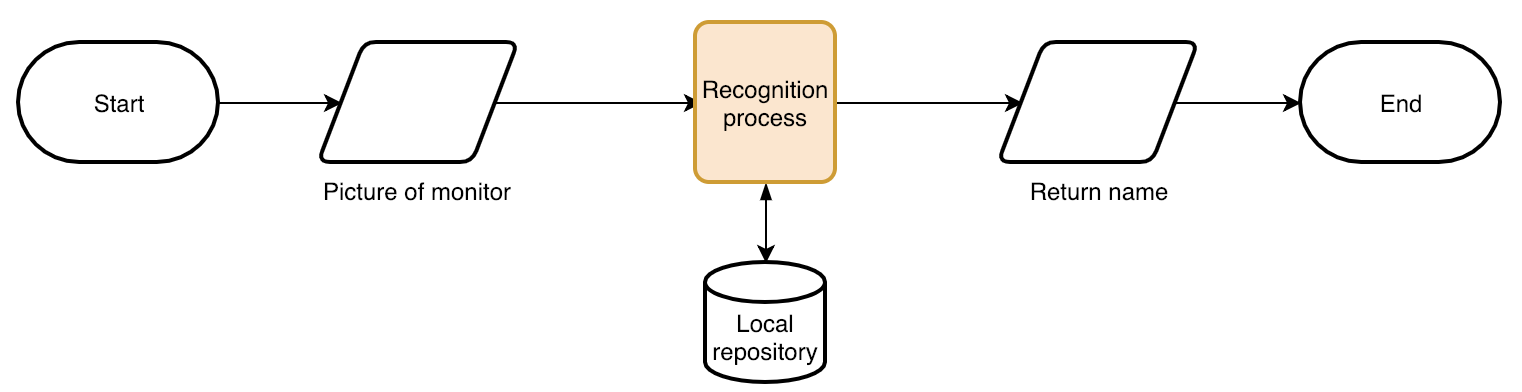
\includegraphics[width=1\textwidth]{Pictures/base_idea_chart.png}
\end{figure}
\newline
Come prima operazione, l'utente scatterà una foto del monitor tramite il telefono, questa nuova immagine verrà processata all'interno della nostra libreria.
La libreria, con l'ausilio di una repository locale, elaborerà questa immagine con le informazioni fondamentali contenute nella repository, per produrre il risultato desiderato.
\Decaa
Andremo quindi a definire:
\begin{itemize}
\item Logica di elaborazione
\item Struttura dei dati di appoggio
\end{itemize}


\newpage
\subsection{Qualità dell'immagine di partenza e considerazioni implementative}
Prima di trarre qualsiasi decisione sulla logica da utilizzare, è necessario comprendere con quale tipologia di dati la nostra libreria andrà a lavorare. Partiamo con un esempio di una immagine del monitor presa da telefono:

\begin{figure}[h!]
  \centering
    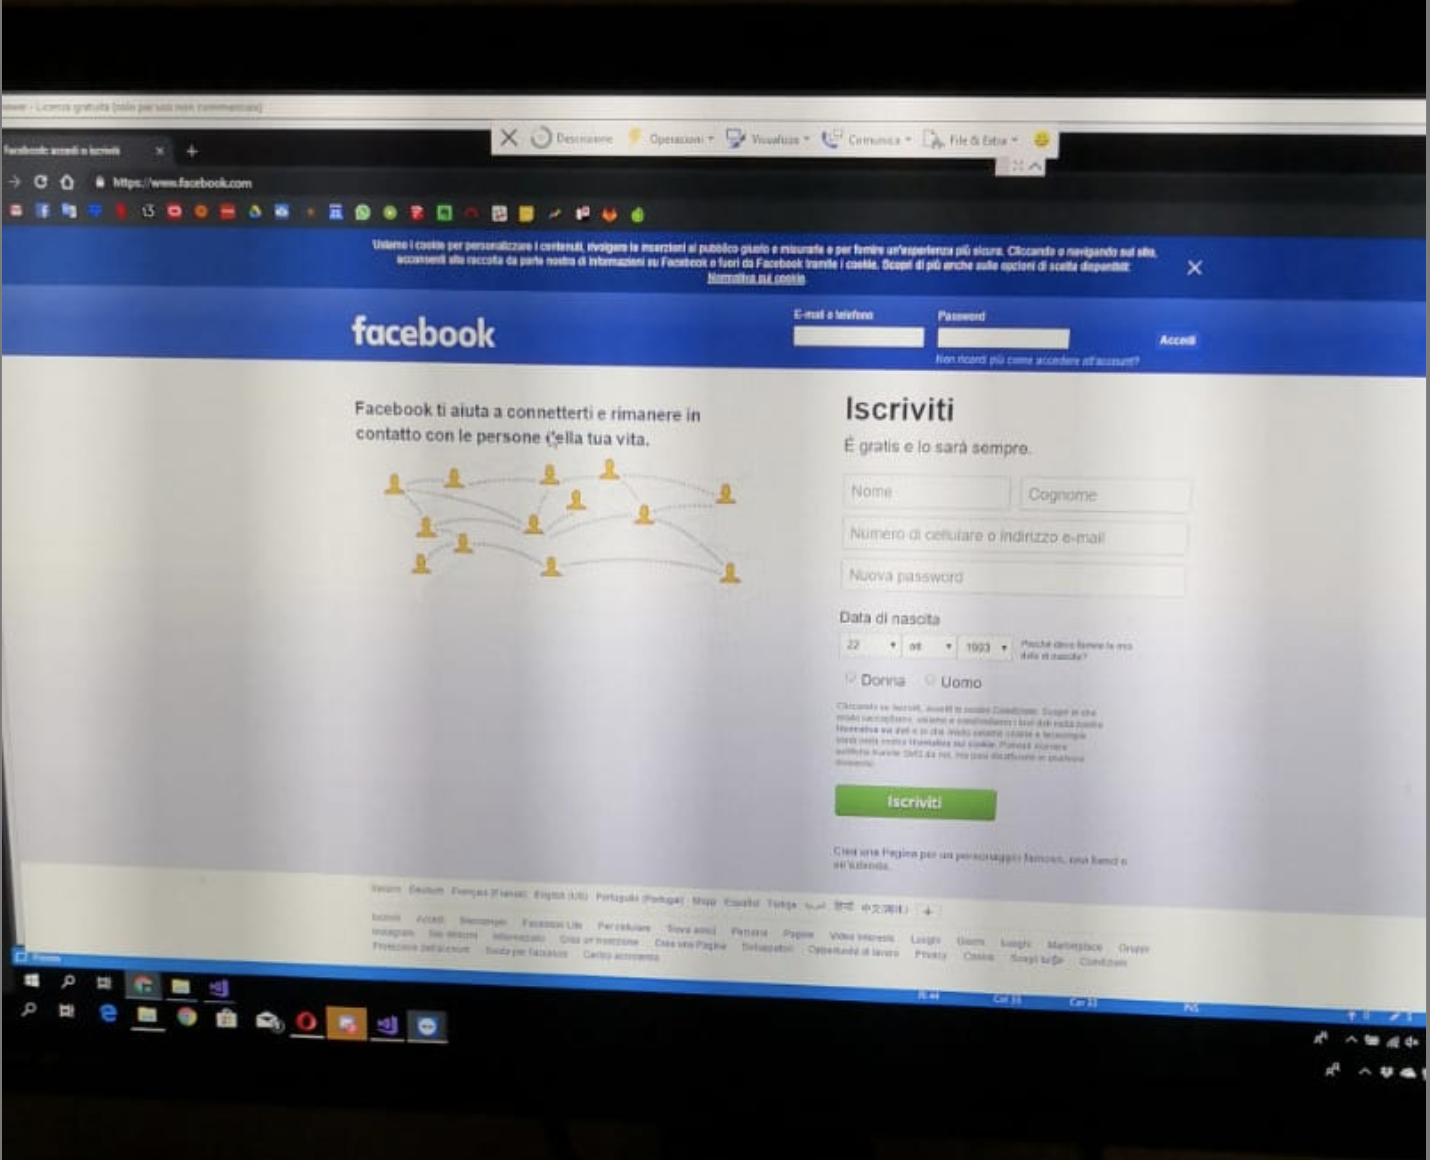
\includegraphics[width=0.8\textwidth]{Pictures/imageToFindTrim.png}
\end{figure}
\newline
Già a colpo d'occhio si può osservare che da una distanza media di 40 cm, si cominciano a perdere parecchi dettagli. Infatti le scritte di testo sono difficilmente leggibili e l'URL della pagina quasi irriconoscibile.
\Decaa
In presenza di questi fattori, ci siamo resi conto che difficilmente saremmo riusciti ad identificare la pagina web tramite riconoscimento ottico dei caratteri. Forse avremmo qualche possibilità con il logo principale, ma assolutamente senza speranze con l'URL.
\Decaa
Abbiamo quindi deciso di optare per una soluzione alternativa, ovvero utilizzare delle tecnologie di computer vision. Nello specifico, utilizzeremo degli algoritmi di feature matching e feature detection. La principale motivazione di questa decisione risulta nel fatto che queste tecnologie sono più robuste, permettendo di ricavare informazioni importanti anche da immagini di questo genere.

\subsection{Definizione logica di implementazione}
\subsubsection{Visione di insieme - logica principale}
A seguire uno schema rappresentativo della logica di implementazione:
\begin{figure}[h!]
  \centering
    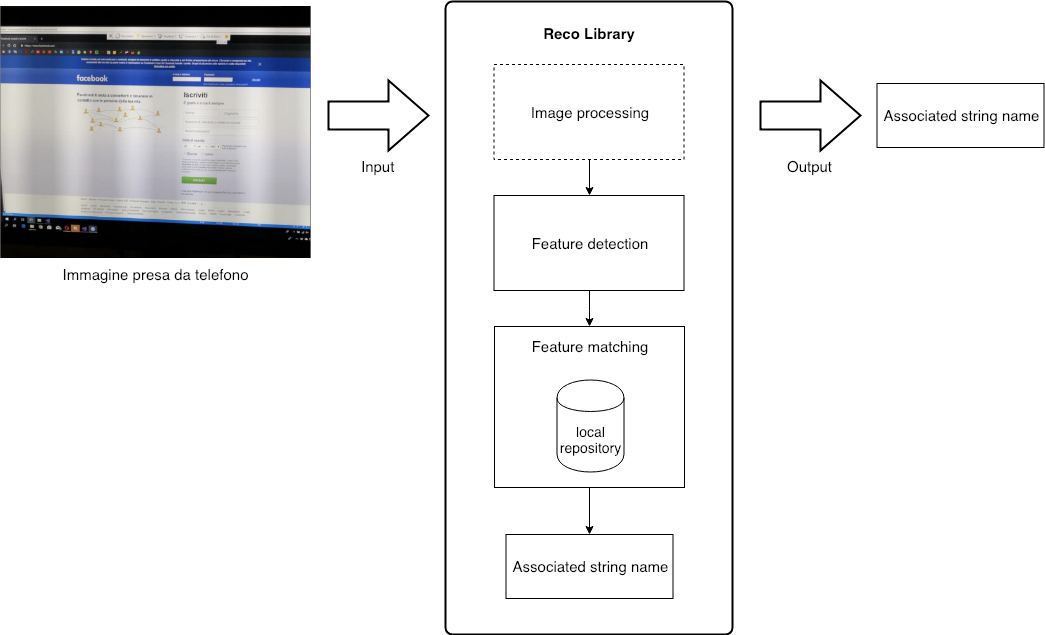
\includegraphics[width=1\textwidth]{Pictures/library_components.png}
\end{figure}
\newline
A partire da una immagine come input, la libreria si occuperà dei seguenti passaggi:
\begin{itemize}
\item Pre-processamenti di immagine (se necessario)
\item Estrapolazione delle caratteristiche dell'immagine
\item Comparazione delle caratteristiche appena trovate, con la repository di caratteristiche locali nel telefono.
\item Ritornare la stringa associata in caso di riscontro.
\end{itemize}

C'è da aggiungere che questa visione globale è valevole sia per modalità desktop, che per versione mobile.

\newpage
\subsubsection{Strutturazione dati}
Per il corretto funzionamento della nostra libreria, è necessario l'ausilio di una struttura dati di appoggio, la così detta repository locale.
\Decaa
Questa repository locale, contiene un insieme di associazioni tra l'immagine fondamentale e la stringa di testo associata.
\begin{figure}[h!]
  \centering
    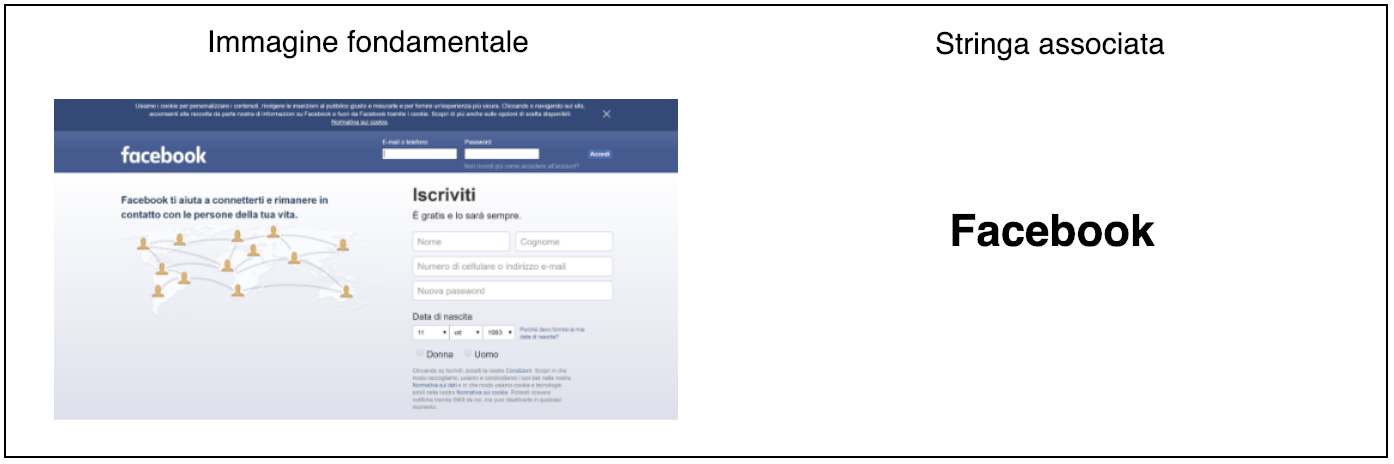
\includegraphics[width=0.8\textwidth]{Pictures/img_fondamentale.png}
\end{figure}
\newline
Questa soluzione però non è la più ottimale, infatti salvando unicamente l'immagine si presentano determinate problematiche:
\begin{itemize}
\item Dimensioni / spazio occupato: salvare ogni singola immagine occupa spazio.
\item Rielaborazione dell'immagine salvata: la libreria per poter svolgere il suo lavoro è obbligata a riprocessare tutte le immagini nella repository.
\item Mancanza delle informazioni fondamentali: in questo modo la repository non sarebbe altro che una raccolta di immagini, senza un valore aggiunto per la libreria
\item Incremento costo computazionale libreria: salvando solo l'immagine, si delega la sua elaborazione nel momento di comparazione a runtime, aumentando drasticamente il tempo necessario per riceve una risposta.
\end{itemize}
Per ottimizzare quanto indicato sopra, abbiamo deciso di strutturare i dati, salvando unicamente le informazioni descrittive dell'immagine fondamentale.
\begin{figure}[h!]
  \centering
    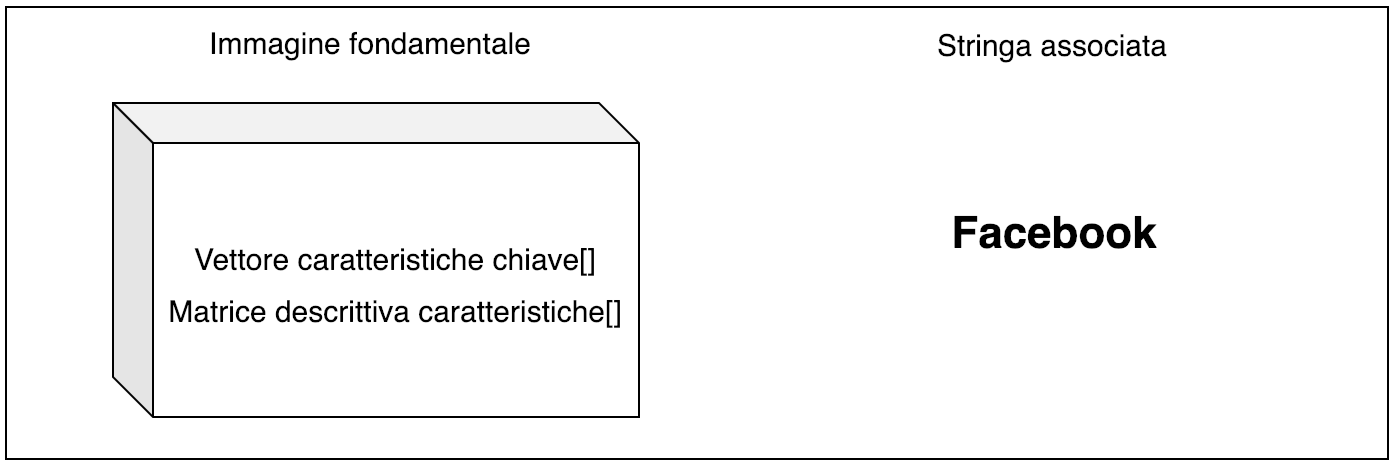
\includegraphics[width=0.8\textwidth]{Pictures/img_fondamentale_preproc.png}
\end{figure}
\newline
Così facendo è anche possibile introdurre questi dati direttamente nel database locale dell'applicativo del committente.

\subsubsection{Algoritmica fondamentale scelta - KAZE e SURF}
Per evadere la logica principale di questa prima parte della nostra libreria, andremo ad utilizzare degli algoritrmi di feature detection e feature matching.
Questi algoritmi andranno ad estrapolare le informazioni inerenti alle immagini utilizzate, e successivamente tramite queste informazioni, identificare delle correlazioni tra le immagini.
Esistono svariati algoritmi di questo tipo, siamo andati quindi ad analizzarne alcuni.
\Decaa
Gli algoritmi che abbiamo testato si chiamano "SURF" (Speeded-Up Robust Features) e "KAZE", ambedue offrono lo stesso risultato, tramite però delle procedure diverse. Per il fine di questo progetto, non siamo entrati troppo nel dettaglio nella comprensione del loro funzionamento (matematico e procedurale), ma bensì abbiamo eseguito delle comparazioni pratiche tra i due. Ulteriori approfondimenti in merito a queste tematiche possono essere trovati nella bibliografia.
\Decaa
Dalla nostra comparazione (sia teorica che empirica) abbiamo tratto le seguenti conclusioni:

\begin{itemize}
\item Velocità feature detection: il SURF è più veloce del KAZE
\item Velocità feature matching: il KAZE è più veloce del SURF
\item Precisione della soluzione: simili, dipende dalle immagini utilizzate.
\end{itemize}

All'interno della nostra libreria, l'esecuzione dell'operazione di feature detection viene svolta una sola volta, ovvero quando viene passata l'immagine presa dal telefono per essere elaborata. Una volta elaborata però, la nostra libreria esegue una fase di ricerca, utilizzando molteplici volte l'operazione di feature matching.
\Decaa
Abbiamo pertanto deciso di utilizzare principalmente l'algoritmo KAZE nella nostra release.

\newpage
\subsubsection{Flusso di lavoro implementativo}
Il flusso di lavoro della nostra libreria si presenta in questo modo:
\begin{figure}[h!]
  \centering
    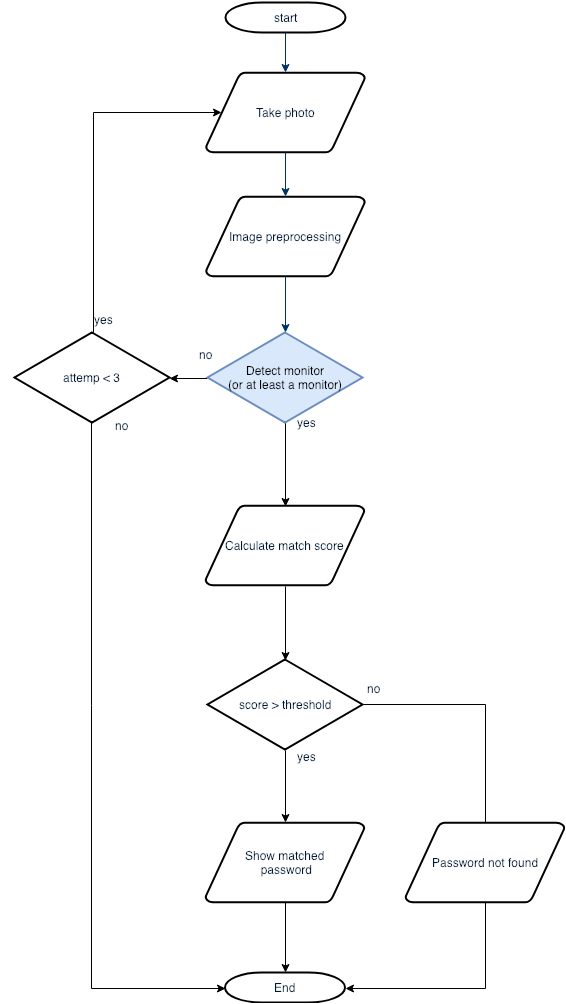
\includegraphics[width=0.8\textwidth]{Pictures/flusso1.png}
\end{figure}
\newline

\section{Design soluzione obbiettivi aggiuntivi}
\subsection{Introduzione elementi di machine learning}
Nel flusso di lavoro implementativo [sezione 4.1.3.4] abbiamo già allocato una posizione logica per l'utilizzo del machine learning.
\Decaa
Nello specifico, abbiamo pensato di utilizzare delle metodologie di classificazione, per svolgere gli obbiettivi aggiuntivi prefissati.

\subsection{Libreria di binding: TensorFlowSharp}
Come prefissato negli obbiettivi aggiuntivi, siamo andati ad utilizzare TensorFlow per svolgere tutti gli aspetti legati alla tematica del machine learning. Purtroppo TensorFlow non dispone dei bindig ufficiali per il linguaggio di programmazione  C\#, siamo quindi andati ad utilizzare un binding non ufficiale, indicatoci direttamente nella pagina web di tensorflow.
\Decaa
Dopo alcune ulteriori ricerche, abbiamo scoperto che la libreria TensorFlowSharp non dispone dei binding per funzionare su mobile. Sarà quindi necessario identificare una soluzione alternativa, come per esempio tensorflow lite.

\subsection{Rilevare la presenza di un monitor nell'immagine}
\subsubsection{La computer vision da sola non è abbastanza...}
Rilevare un determinato oggetto all'interno di una foto, risulta essere un problema complesso. Ancora più complesso utilizzando unicamente tecnologie di computer vision. Infatti, per risolvere questo problema con solo la computer vision, bisognerebbe svolgere svariate operazioni, come per esempio:
\begin{itemize}
\item Preparare in maniera corretta l'immagine, ridimensionandola e portandola ad una colorazione su scale di grigio;
\item Tramite sistemi di sfocatura o ritocco di immagine, enfatizzare il più possibile i contorni all'interno della foto;
\item Utilizzare degli algoritmi di rilevamento dei contorni per rilevare delle forme a partire dai bordi;
\item Implementare una logica per "escludere" le forme che non sono rettangolari nella foto;
\item Indovinare se uno o più di questi rettangoli sono dei monitor;
\end{itemize}
Come si può ben notare, i passaggi da eseguire sono molti, alcuni di essi complessi ed altri ancora sono poco definiti. Per questo motivo abbiamo deciso di risolvere il problema mediante machine learning.
\subsubsection{Introduzione/utilizzo classificatori}
Per identificare il monitor, andremo ad utilizzare un classificatore, ovvero un componente utilizzato nel machine learning per riconoscere o classificare un determinato oggetto, in una classe (tipo) conosciuta dal classificatore.
\Decaa Per fare questo, abbiamo deciso di utilizzare un classificatore basato su una rete neurale convoluzionale. Questa rete neurale, che ricorda vagamente il funzionamento stesso del nostro cervello, data una immagine di input è in grado di classificarla in determinate classi (tipologie) a lei conosciuta.
\Decaa
Andremo quindi ad interagire con uni di questi classificatori, provando in un primo momento a modificarlo, tramite il train (allenamento) dell'ultimo layer, per vedere cosa ne esce. Successivamente proveremo ad integrare uno di questi classificatori all'interno della nostra libreria, così che possa, data l'immagine di input, determinare se nella foto è presente un monitor.
\Decaa
A livello didattico, sarà interessante comprendere come si introduce, modifica o utilizza un classificatore già addestrato e pronto all'uso, all'interno della nostra soluzione.

\subsection{Studio/creazione di un classificatore personalizzato}
Un'ulteriore valore aggiunto che può essere inserito all'interno della nostra libreria, potrebbe essere quello di rilevare la presenza di eventuali loghi di pagine web conosciute. Per fare questo, sarà necessario analizzare alcuni componenti fondamentali per la creazione di un classificatore, più nel dettaglio, di un classificatore basato su rete neurale.\Decaa
Proveremo a creare, partendo da zero, tutto ciò che è necessario per sviluppare un classificatore personalizzato per rispondere alla nostra necessità. Sarà quindi necessario svolgere le seguenti operazioni:
\begin{itemize}
\item Trovare o costruire un dataset per l'apprendimento del nostro classificatore.
\item Pulire i dati raccolti in modo che possano essere utilizzati correttamente
\item Creare il classificatore, allenandolo con i dati raccolti
\item Testarne la sua accuratezza
\end{itemize}

\chapter{Implementazione soluzioni}%rob
Per facilitare la comprensione degli elementi del progetto (Computer Vision, Machine Learning, ecc...) abbiamo deciso in un primo momento di sviluppare le funzionalità della libreria per desktop, in quanto erano per noi più facili da testare. In un secondo momento, abbiamo programmato un'applicazione Demo per dimostrare la portabilità della libreria su dispositivi mobile.

\section{Implementazione obbiettivi iniziali}%rob
Per lo sviluppo della nostra soluzione, abbiamo pensato di creare un oggetto semplice, che abbiamo chiamato Record. L'idea  di base, è che questo oggetto contenga le informazioni ricavate da un esecuzione di un algoritmo di feature detection, in modo che il processo di confronto con altre immagini non richieda troppe risorse. 

\begin{lstlisting}[language=C]

    [Serializable()]
    public class Record
    {
        ///////////////////////////////////////////////////////////
        ///Fields
        //////////////////////////////////////////////////////////

        private readonly String name;
        private readonly VectorOfKeyPoint keyPoint;
        private readonly Mat descriptors;

        public VectorOfKeyPoint KeyPoints { get { return keyPoint; } }
        public String Name { get { return name; } }
        public Mat Descriptors { get { return descriptors; } }

        // Private constructor
        private Record(String name) {
            this.name = name;
            this.keyPoint = new VectorOfKeyPoint();
            this.descriptors = new Mat();
        }
    ...
\end{lstlisting}

Questa classe espone un solo metodo, la creazione di un nuovo Record:

\begin{lstlisting}[language=C]
public static Record CreateFromImage(String path, String name) {
            // new Record
            Record newRecord = new Record(name);

            //Preprocessing of the image
            Mat image = CvInvoke.Imread(path, ImreadModes.Color);
            UMat uImage = image.GetUMat(AccessType.Read);
            KAZE surf = new KAZE();
            surf.DetectAndCompute(uImage, null, newRecord.keyPoint, newRecord.descriptors, false);

            return newRecord;
        }
\end{lstlisting}

Come mostrato sopra, il metodo restituisce un nuovo record. Al Record è collegato una stringa "name" che serve a recuperare il valore corrispondente dell'immagine (come facebook, netflix, o anche l'URL direttamente, dipenderà da come vorrà essere utilizzata la libreria). Prima di restituire l'oggetto, viene eseguito il metodo di feature detection e salvati i relativi dati. Questo metodo è pensato per ampliare il database locale qualora i dati precaricati non siano sufficienti o quando l'utente deve riconoscere siti personalizzati. 

La libreria vera e propria è la classe Reco.cs. Espone poche API atte a risolvere il problema proposto, come ad esempio il metodo per il recupero del nome data un'immagine in input. 

Attualmente date le tempistiche e lo scopo della libreria (conoscere quali strumenti si possono utilizzare per risolvere questo tipo di problemi) i Record sono serializzati e salvati localmente. Quando si utilizza la libreria si può richiamare un metodo load per caricare il file contenente i record in memoria. In futuro, chiaramente si può migliorare questa gestione utilizzando ad esempio un componente come LINQ presente nel framework .NET.
Sono presenti due funzioni per l'aggiunta e rimozione di record:


\begin{lstlisting}[language=C]
public bool AddImage(String imagePath, String name) {
            Record record;
            try
            {
                record = Record.CreateFromImage(imagePath, name);
                records.Add(record);
                return true;
            }
            catch (Exception e) {
                return false;
            }
            
        }
        
        /// <returns>Return true if the Record is found and correctly removed from the repository, else false</returns>
        public bool RemoveImage(String name) {
            return records.Remove(records.Find(r=>r.Name.Equals(name)));
        }
\end{lstlisting}

Abbiamo programmato un metodo chiamato GetNameList che, dato il percorso di un'immagine, genera un oggetto della classe Record, senza nessun nome associato, dopodichè utilizza le proprietà calcolate per generare un valore di score per ogni confronto. Sfruttando il metodo presente nella classe Utility, Sort List (che abbiamo implementato per ordinare la lista in base allo score di ogni confronto) restituisce una lista ordinata di coppie chiave-valore. La chiave è il nome registrato insieme al record, mentre il valore rappresenta lo score risultante dalla comparazione. In questo modo, si ottiene una lista di nomi per il quale il primo elemento è l'immagine con più punti in comune con quella in ingresso. 

Il sort è effettuato in questo modo:

\begin{lstlisting}[language=C]
  public static void sortList(List<KeyValuePair<string, int>> list) {
            list.Sort(
                delegate(KeyValuePair<string,int> pair1,
                KeyValuePair<string,int> pair2) {
                    return pair1.Value.CompareTo(pair2.Value);
                }
            );
          
        }
\end{lstlisting}

Il metodo invece si presenta così:

\begin{lstlisting}[language=C]
 private List<KeyValuePair<String, int>> GetNameList(String imagePath)
        {
            Record processingRecord = Record.CreateFromImage(imagePath, "");
            var resultList = new List<KeyValuePair<String, int>>();
            VectorOfVectorOfDMatch matches = new VectorOfVectorOfDMatch();
            int k = 2;
            double uniquenessThreshold = 0.8;
            Mat mask = new Mat();

            records.ForEach(e => {
                using (Emgu.CV.Flann.LinearIndexParams ip = new Emgu.CV.Flann.LinearIndexParams())
                using (Emgu.CV.Flann.SearchParams sp = new SearchParams())
                using (DescriptorMatcher matcher = new FlannBasedMatcher(ip, sp))
                {
                    matcher.Add(e.Descriptors);

                    matcher.KnnMatch(processingRecord.Descriptors, matches, k, null);
                    mask = new Mat(matches.Size, 1, DepthType.Cv8U, 1);
                    mask.SetTo(new MCvScalar(255));
                    Features2DToolbox.VoteForUniqueness(matches, uniquenessThreshold, mask);

                    // Calcluate the score based on matches size
                    int score = 0;
                    for (int i = 0; i < matches.Size; i++)
                    {
                        if (mask.GetData(i)[0] == 0) continue;
                        foreach (var item in matches[i].ToArray())
                            ++score;
                    }

                    // Add score and record's name to the map
                    resultList.Add(new KeyValuePair<string, int>(e.Name, score));
                }
            });

            Utility.sortList(resultList);
            return resultList;
        }
\end{lstlisting}
Per il confronto delle features delle immagini, esistono diverse possibilità. La prima soluzione è la più semplice ma naturalmente la meno efficace, si utilizza un Brute-Force Matcher. Prende in esame un descrittore di una feature della prima immagine e la confronta con il descrittore di ogni feature rilevata nella seconda. Calcola quindi una distanza utilizzando una determinata funzione e ritorna quella più vicina. Nella nostra libreria però noi abbiamo usato il FLANN Based Matcher. FLANN\cite{flann}, acronimo di Fast Library for Approximate Nearest Neighbour, è una libreria contenente algoritmi di ricerca ottimizzati di nearest neighbour. In OpenCV, l'oggetto Flann Matcher riceve in ingresso due parametri, index\_params e search\_params. Il primo indica l'algoritmo da utilizzare (ne sono disponibili diversi) ognuno con le sue particolarità. La scelta dipende da quante risorse e quanto tempo si vuole dedicare a questa operazione. Il secondo parametro indica quante volte devono essere attraversati gli alberi nell'indice. Più volte significa più precisione, ma naturalmente anche più tempo di elaborazione. 

\subsection{Test e risultati}%rob
\subsubsection{test di unità della libreria}
Durante lo sviluppo abbiamo utilizzato la libreria fornita da Microsoft per i test d'unità. Per tutti i componenti sono stati sviluppati i test a livello desktop. Dato i tempi limitati i test per le piattaforme mobile non sono stati eseguiti. 

Di seguito un esempio di test d'unità della classe Record:

\begin{lstlisting}
  [TestClass]
    public class RecordTest
    {

        [TestMethod]
        [ExpectedException(typeof(ArgumentException))]
        public void createFromNotFoundTest() {
            Record emptyRecord = Record.CreateFromImage("Resources/notFoundImage.png","notFoundImage"); 
        }

        [TestMethod]
        public void createFromImageTest(){
            Record record = Record.CreateFromImage("Resources/testImage1.png", "testImage1");
            Assert.IsNotNull(record);
        }
    }
\end{lstlisting}

I test per la libreria invece sono strutturati in questo modo:

\begin{lstlisting}
using Microsoft.VisualStudio.TestTools.UnitTesting;
using System;
using RecoLibrary;
using System.Collections.Generic;

namespace RecoTest
{
    [TestClass]
    public class RecoTest
    {
        [TestInitialize]
        public void TestInitialize()
        {
            Reco.GetInstance().purgeRecoInstance();
        }

        [TestMethod]
        public void AddImageAndSaveTest()
        {
            Assert.IsFalse(Reco.GetInstance().AddImage("notFound.png", "notFoundImage"));
            Assert.IsTrue(Reco.GetInstance().AddImage("Resources/testImage1.png", "testImage1"));
            Reco.GetInstance().AddImage("Resources/testImage2.png", "testImage2");
            Reco.GetInstance().AddImage("Resources/testImage3.png", "testImage3");
            Reco.GetInstance().AddImage("Resources/testImage4.png", "testImage4");
            Assert.AreEqual(4, Reco.GetInstance().GetNumberOfRecords());
            Assert.IsTrue(Reco.GetInstance().Save("Resources/sampleRepository.bin"));
        }
        [TestMethod]
        public void GetInstanceAndLoadTest()
        {
            //Check consistency of Reco instance and records field without input file
            Assert.IsNotNull(Reco.GetInstance());
            Assert.AreEqual(0,Reco.GetInstance().GetNumberOfRecords());

            //load a repository.bin test file
            Assert.IsTrue(Reco.GetInstance().Load("Resources/sampleRepository.bin"));

            //Check consistency of Reco instance and records field with input test file
            Assert.AreEqual(4, Reco.GetInstance().GetNumberOfRecords());

        }

        [TestMethod]
        public void GetNameTest()
        {
           Reco.GetInstance().Load("Resources/sampleRepository.bin");
           string name=Reco.GetInstance().GetName("Resources/imageToFind.jpeg");
           Assert.AreEqual(name, "testImage1");
        }

        [TestMethod]
        public void GetNNameTest()
        {
            Reco.GetInstance().Load("Resources/sampleRepository.bin");
            List<string> names = Reco.GetInstance().GetNNames("Resources/imageToFind.jpeg",2);
            Assert.AreEqual(names[0], "testImage1");
            Assert.AreEqual(names[1], "testImage2");
        }

        [TestMethod]
        public void RemoveTest()
        {
            Reco.GetInstance().Load("Resources/sampleRepository.bin");
            Assert.IsTrue(Reco.GetInstance().RemoveImage("testImage1"));
        }
        ...
\end{lstlisting}

Prima di ogni test è eseguito il metodo annotato con "TestInitialize" che esegue un purge dell'istanza contenente i Record salvati in precedenza. Gli altri metodi verificano invece l'aggiunta di immagini alla libreria, la rimozione di immagini, il recupero del nome data un'immagine in input e il recupero dei nomi dei record più probabili data un'immagine in input.
\Decaa
In termini di precisione la libreria funziona molto bene anche eseguendo la foto in un ambiente scuro, girando la fotocamera o da lontano. Le prestazioni invece dipendono maggiormente dagli algoritmi utilizzati. Il primo è quello di feature detection, a livello desktop abbiamo potuto testare il KAZE e il SURF. 
L'algoritmo più veloce è quello migliore nell'ambito di matching (e non in fase di detection), KAZE. Nei test desktop con una lista di Record di una decina di immagini si riesce ad avere una risposta nell'ordine di 500-600 ms. Con quattro immagini il tempo arriva a circa 450-550ms. Il sistema quindi è abbastanza prestante ma la scalabilità non è garantita. Per migliorare i tempi di risposta bisogna conoscere meglio gli algoritmi di matching e capire quale sarebbe meglio in caso di database con un paio di centinaia di immagini.

\subsubsection{Risultati ottenuti}
Per testare i risultati ottenuti dalla nostra libreria, siamo andati ad eseguire alcune prove pratiche. Nello specifico, abbiamo utilizzato delle foto prese da telefono, per testare velocità e risultato di questa prima parte della libreria.\Decaa
Per questioni di spazio e di completezza, andremo a sviluppare nel dettaglio un caso pratico, per tirare le somme generali di prestazione.Partendo da una stessa immagine, siamo andati a provare nella pratica i due algoritmi di feature matchine e feature detection presi in analisi: KAZE e SURF.
\Decaa
Partendo da una stessa immagine di input:
\newline
\begin{figure}[h!]
  \centering
    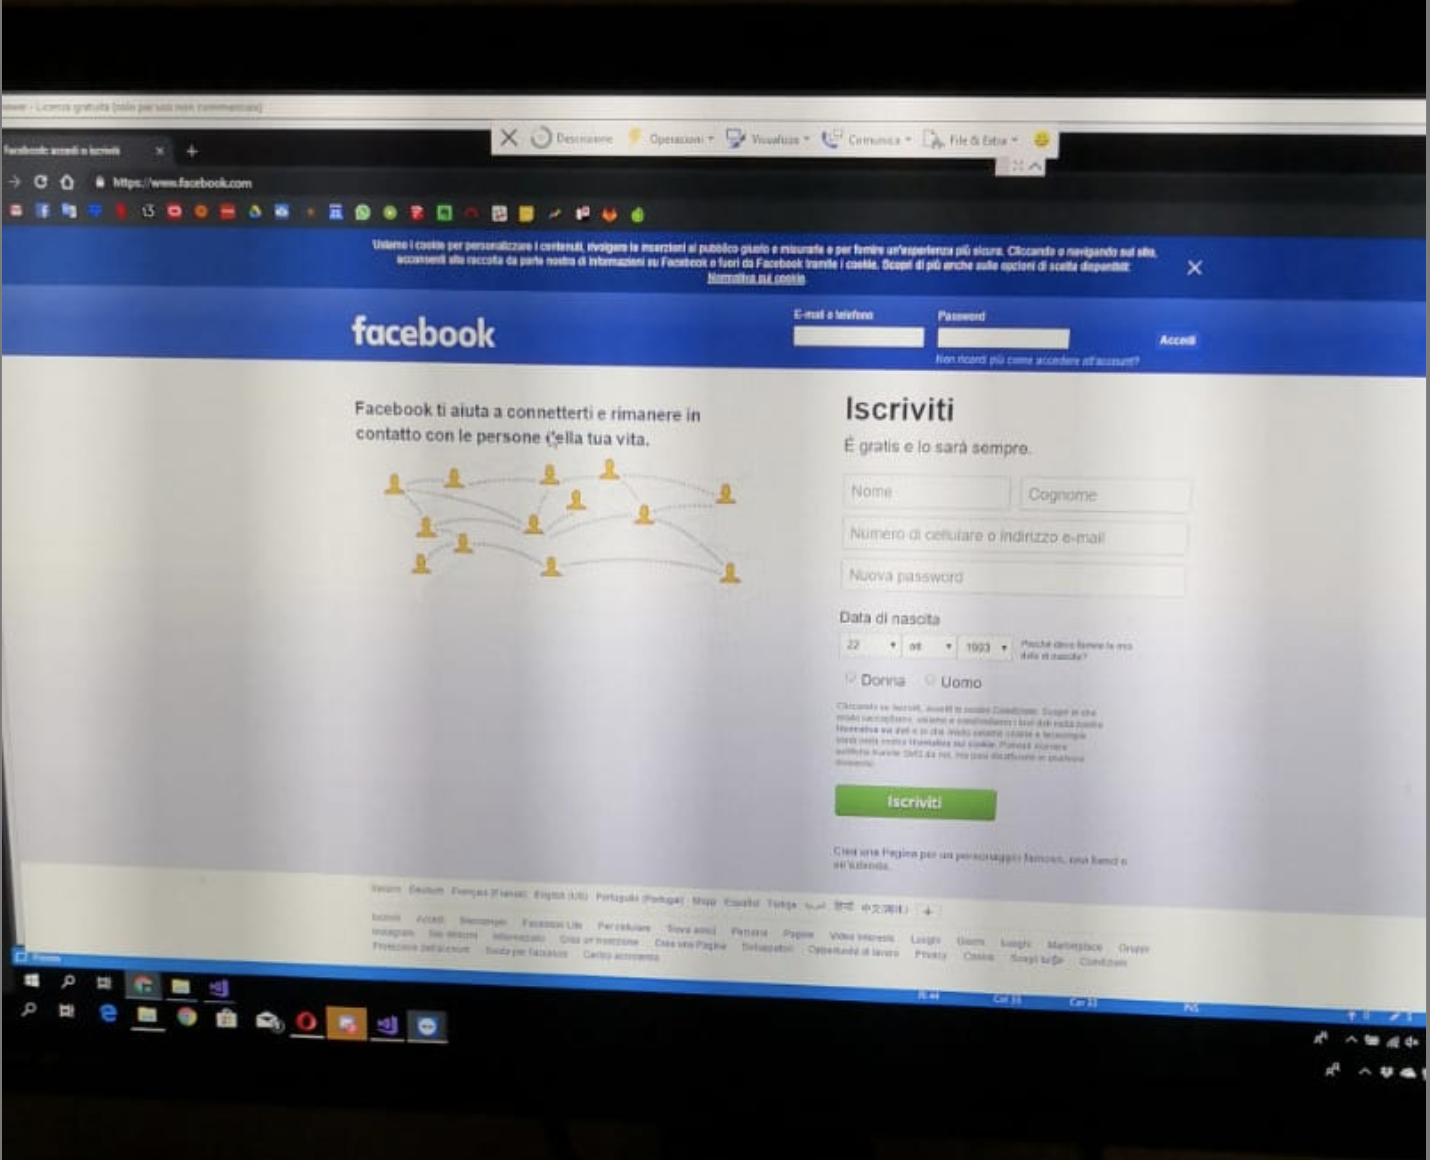
\includegraphics[height=0.3\textwidth]{Pictures/imageToFindTrim.png}
\end{figure}
\newline
Iniziando con l'algoritmo KAZE, il risultato ottenuto è questo:
\begin{figure}[h!]
  \centering
    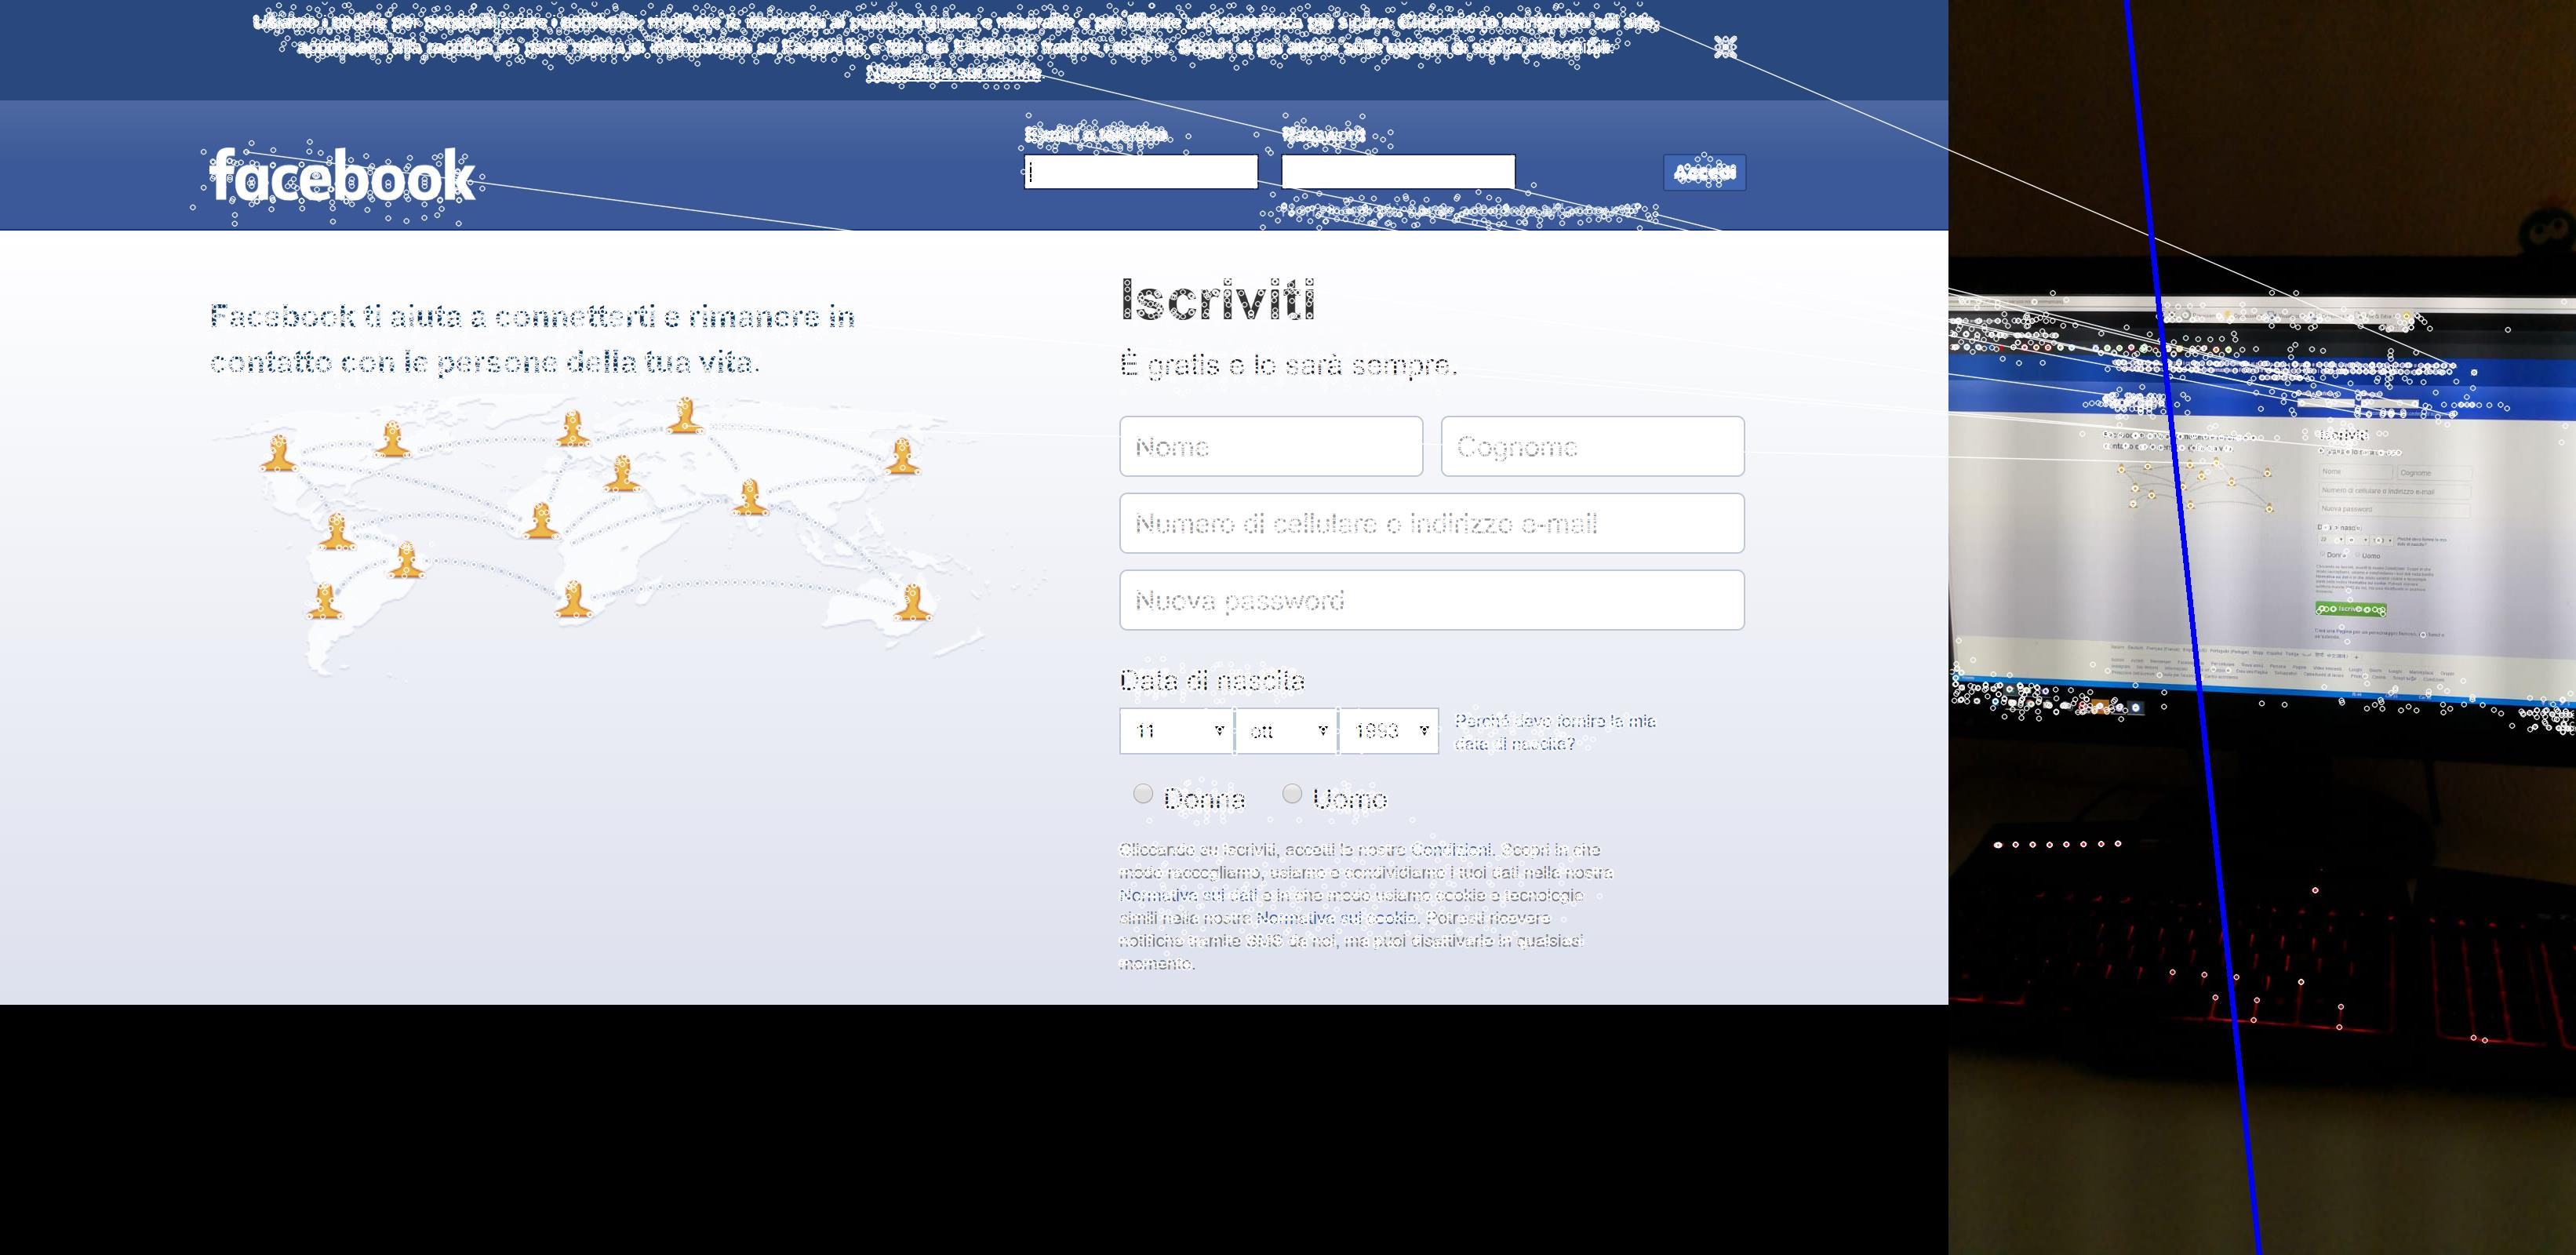
\includegraphics[width=0.8\textwidth]{Pictures/resultKAZE.jpeg}
\end{figure}
\newline
Mentre che con l'algoritmo SURF si ottiene:
\begin{figure}[h!]
  \centering
    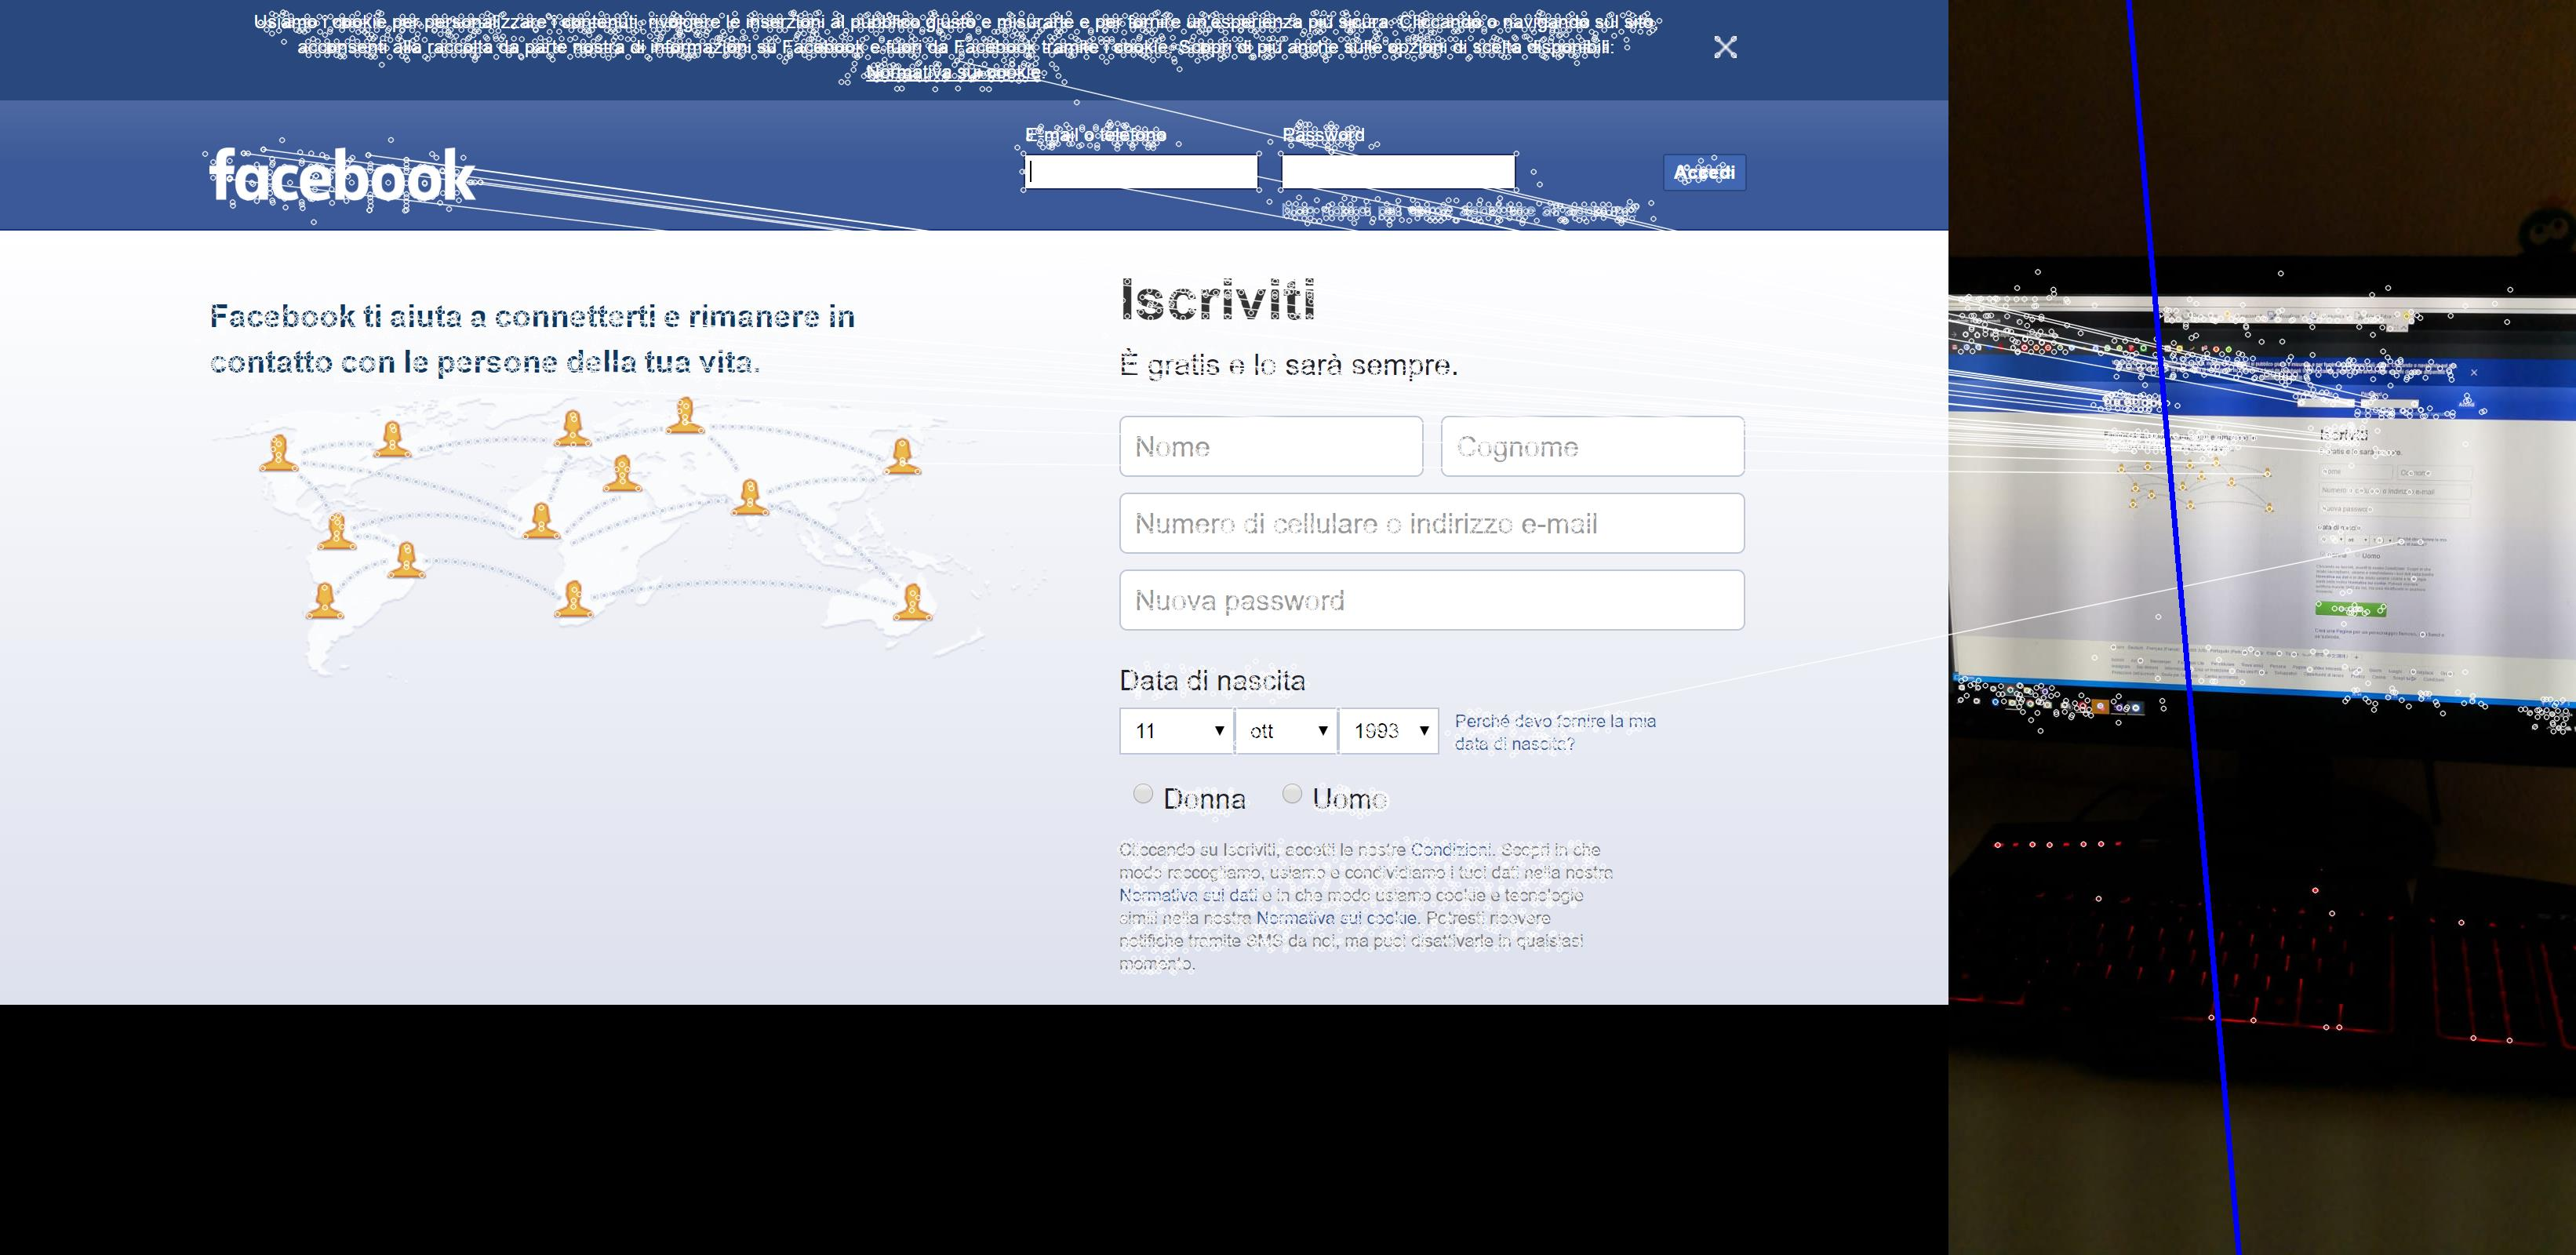
\includegraphics[width=0.8\textwidth]{Pictures/resultSURF.jpeg}
\end{figure}
\newline
Come si può notare, ambedue hanno trovato una corrispondenza con l'immagine fondamentale di "Facebook", con però dei riscontri diversi.
\Decaa
Infatti, parlando proprio dei riscontri ottenuti, ecco i risultati dei test precedenti:
\newline
Matching score con KAZE:
\begin{figure}[h!]
  \centering
    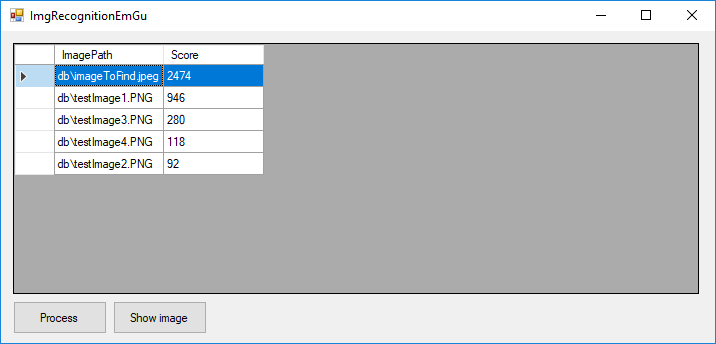
\includegraphics[width=1\textwidth]{Pictures/Matching_scores_KAZE.PNG}
\end{figure}
\newline
Matching score con SURF:
\begin{figure}[h!]
  \centering
    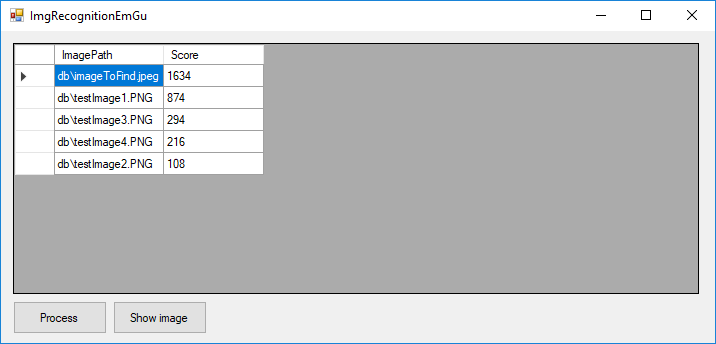
\includegraphics[width=1\textwidth]{Pictures/Matching_scores_SURF.PNG}
\end{figure}
\newline
Come analizzato in precedenza, possiamo vedere che l'algoritmo KAZE ha trovato in generale un numero di riscontri più alto rispetto all'algoritmo SURF. Addirittura più di 800 riscontri sono stati trovati con la stessa immagine di input.\Decaa
Parlando di tempistiche, dopo svariate prove abbiamo constatato che, il tempo di risposta della nostra libreria è di circa 500ms per 10 elementi della repository. Possiamo pertanto stimare una media di 50ms per ogni elemento da cercare. Purtroppo questa è puramente una stima analitica, infatti al crescere della repository, è possibile che i tempi di risposta aumentino. \Decaa
Come prima versione di questa libreria, i tempi di risposta sono accettabili. Da notare che la libreria attualmente è unicamente in uno stato funzionale, c'è ancora molto margine di manovra per delle ottimizzazioni, sia per la gestione della memoria, sia per l'aumento delle prestazioni generali.

\newpage
\section{Implementazione obbiettivi aggiuntivi}%rob
\subsection{Utilizzo del machine learning}
Per poter testare gli strumenti per l'utilizzo di Machine Learning, abbiamo implementato un semplice metodo che ritorna true se nell'immagine è presente un monitor (o uno schermo). Abbiamo usato Tensorflow per addestrare l'ultimo layer di una rete neurale già preaddestrata, dando in pasto al classificatore un centinaio di immagini contenenti monitor o schermi e altrettante senza monitor. Con così poche immagini di test il classificatore non funzionava correttamente. Restituiva infatti, come ci si può aspettare, che il monitor non era presente. Il dato che però tornava utile era la percentuale di confidenza della risposta. Infatti se il monitor era presente, la confidenza passava da un 99\% a un 94\%. 
Abbiamo trovato in rete però un modello già addestrato che tra i nodi di output presenta la label "monitor", perfetto per i nostri test. Il modello si chiama MobileNetV2 ed ha un'architettura ottimizzata per i dispositivi mobili. Di seguito è mostrato un grafico che mette a confronto diverse reti neurali esistenti.
\Decaa
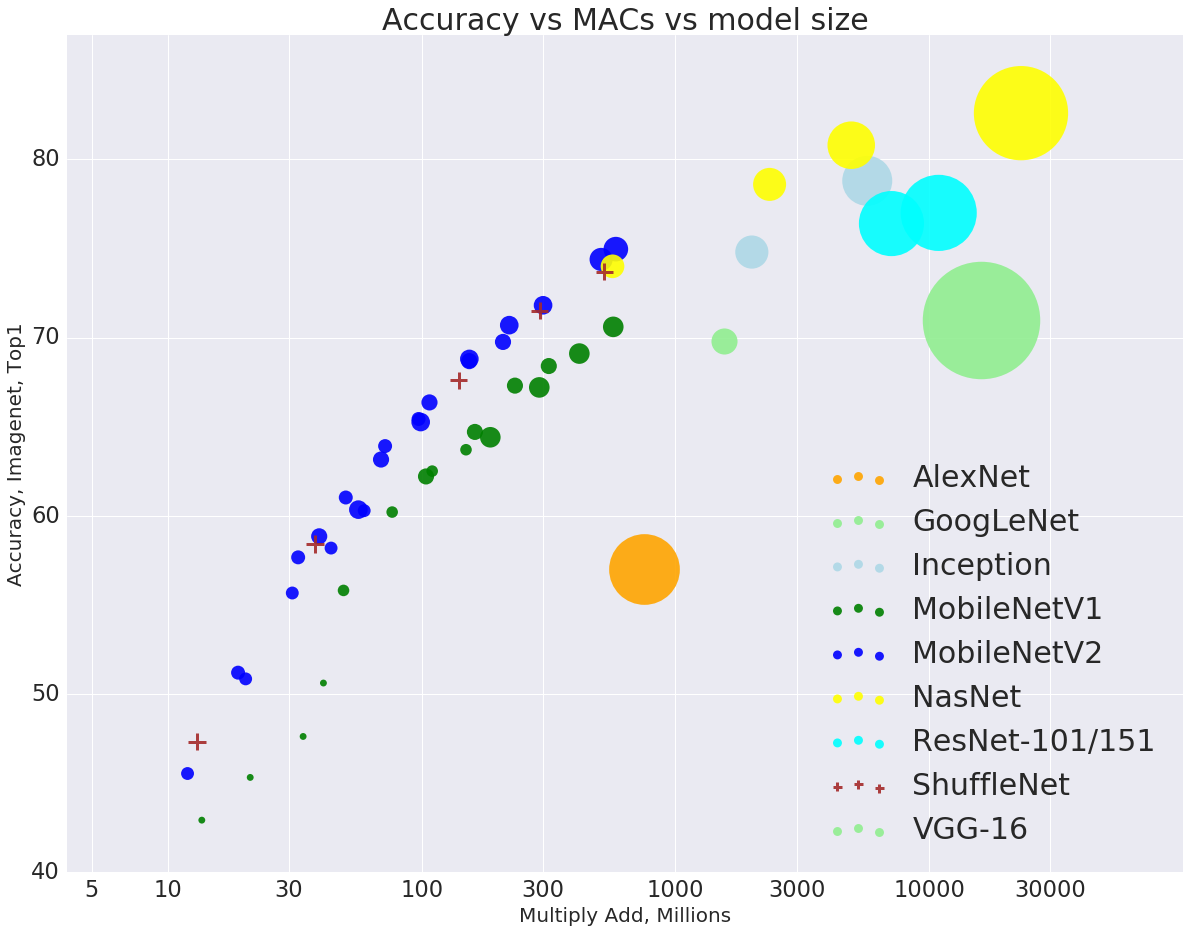
\includegraphics[width=\textwidth]{Pictures/accuracy.PNG}
\Decaa
I file da caricare nell'applicazione sono quindi solamente due: il modello, e la lista delle label. 

\begin{lstlisting}
        public Boolean isMonitor(String imagePath) {
            var graph = new TFGraph();
            // Load the serialized GraphDef from a file.
            var model = File.ReadAllBytes(modelFile);

            graph.Import(model, "");

            var tensor = ImageUtil.CreateTensorFromImageFile(imagePath, TFDataType.Float);
            var session = new TFSession(graph);
            
                var labels = File.ReadAllLines(labelsFile);
                var runner = session.GetRunner();
                runner.AddInput(graph["input"][0], tensor);
                runner.Fetch(graph["MobilenetV2/Predictions/Reshape_1"][0]);

                var output = runner.Run();

                // Fetch the results from output:
                TFTensor result = output[0];

                bool jagged = true;

                var bestIdx = 0;
                float p = 0, best = 0;

                // You can get the data in two ways, as a multi-dimensional array, or arrays of arrays, 
                // code can be nicer to read with one or the other, pick it based on how you want to process
                // it
                if (jagged)
                {
                    var probabilities = ((float[][])result.GetValue(jagged: true))[0];
                    for (int i = 0; i < probabilities.Length; i++)
                    {
                        if (probabilities[i] > best)
                        {
                            bestIdx = i;
                            best = probabilities[i];
                        }
                    }
                }
                else
                {
                    var val = (float[,])result.GetValue(jagged: false);

                    // Result is [1,N], flatten array
                    for (int i = 0; i < val.GetLength(1); i++)
                    {
                        if (val[0, i] > best)
                        {
                            bestIdx = i;
                            best = val[0, i];
                        }
                    }
                }
                Console.WriteLine($"best match: [{bestIdx}] {best * 100.0}% {labels[bestIdx]}");
                
            return isMonitorOrSimilarLabel(labels[bestIdx]);
        }

        private bool isMonitorOrSimilarLabel(string v)
        {
            return v.Equals("Monitor", StringComparison.OrdinalIgnoreCase) ||
                v.Equals("Screen", StringComparison.OrdinalIgnoreCase) ||
                v.Equals("television", StringComparison.OrdinalIgnoreCase) ||
                v.Equals("website", StringComparison.OrdinalIgnoreCase);
        }

        static void ModelFiles(string dir)
        {
            modelFile = "Resources/model/mobilenet_v2_1.0_224_frozen.pb";
            labelsFile = "Resources/model/labels.txt";
            if (File.Exists(modelFile) && File.Exists(labelsFile))
                return;
        }
\end{lstlisting}

Per poter testare queste tecnologie in Xamarin abbiamo cercato una libreria cross-platform. Purtroppo la ricerca ha dimostrato che in questo ambito soluzioni multi-piattaforma non esistono o, se invece ci sono, funzionano male. Tensorflow ha il supporto sia per iOS che per Android, ma solo per lo sviluppo nativo. 
Per poter usare qualcosa anche con Xamarin abbiamo trovato una libreria chiamata TensorFlowSharp che sono i bindings di C\# per Tensorflow.

\subsection{Creazione di un classificatore con rete neurale}
In questa sezione, cercheremo di creare un classificatore con una rete neurale convoluzionale, con lo scopo di identificare il logo di un brand tra quelli "imparati" dal classificatore. Nello specifico, prenderemo come esempio 14 loghi conosciuti, ovvero:
\begin{multicols}{3}
\begin{itemize}
\item Apple
\item Facebook
\item Google
\item Youtube
\item Twitter
\item Microsoft
\item Reddit
\item Stack overflow
\item Wikipedia
\item Yahoo
\item Gmail
\item Hotmail
\item Amazon
\item Instagram
\end{itemize}
\end{multicols}

\subsubsection{Costruzione di un dataset}
Prima di tutto, per costruire un classificatore, è fondamentale ricavare un gran numero di dati, da inserire in un dataset.
In rete è possibile trovare tantissimi dataset generici e open source, utili per creare classificatori di ogni genere.
Nel nostro caso però, non abbiamo trovato alcun dataset già esistente contenente dei loghi di pagine web. Pertanto lo abbiamo creato noi.\Decaa
Tramite l'applicazione "Google-Image-Download" già descritta in precedenza, siamo andati a scaricare 100 immagini per ognuno dei loghi sopracitati, ordinati poi con un sistema di directory. Purtroppo però, per il nostro classificatore, 100 immagini non bastano nemmeno per cominciare. Per aumentare il numero di immagini a nostra disposizione, possiamo crearne delle nuove a partire da quelle appena scaricate, modificandole tramite operazioni algebriche di: ridimensionamento, rotazione e stiratura delle immagini. Per fare questo, è stato utilizzato uno script in python.
\begin{lstlisting}
mport sys
import Augmentor

folder_name='folder'
p= Augmentor.Pipeline(source_directory=folder_name,save_format="png")
p.flip_left_right(0.5)
p.black_and_white(0.1)
p.gaussian_distortion(probability=0.4, grid_width=7, grid_height=6
                      , magnitude=6, corner="ul", method="in", mex=0.5, mey=0.5, sdx=0.05, sdy=0.05)

p.rotate(0.3, 10,10)
p.skew(0.4,0.5)
p.skew_tilt(0.6,0.8)
p.skew_left_right(0.5, magnitude=0.8)
p.sample(100)
\end{lstlisting}
Così facendo, siamo riusciti ad arrivare a circa 14'000 immagini per allenare la nostra rete.
Alcune di queste immagini potrebbero essere troppo poco chiare, per questo motivo è sempre bene dare uno sguardo visivo al dataset, per una superficiale rimozione di eventuali elementi anomali.

\subsubsection{Preparazione del dataset}
Per la costruzione del nostro classificatore, dobbiamo suddividere il dataset appena creato in una struttura di cartelle definita.
A partire da una directory di origine, chiamata dataset, creare due nuove cartelle: "train" e "test". All'interno di queste due cartelle, bisogna definire un numero di cartelle pari alle classi che il classificatore dovrà riconoscere. Nel nostro caso, 14 cartelle chiamate con il nome del brand da riconoscere.
La struttura dovrebbe presentarsi in questo modo:
\begin{figure}[h!]
  \centering
    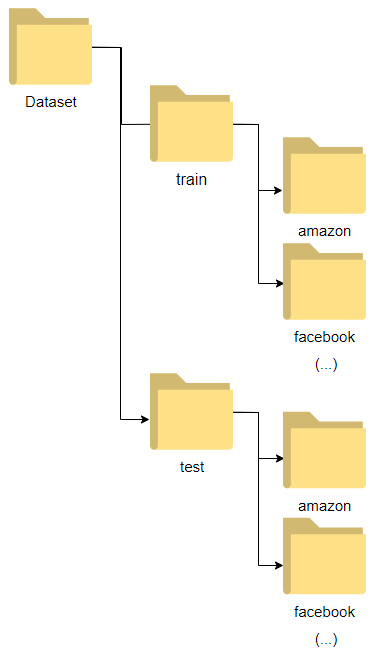
\includegraphics[width=0.4\textwidth]{Pictures/keras_tree.PNG}
\end{figure}
\newline
Infine, spostare 2/3 delle immagini ordinate per classe, all'interno della cartella "train" ed il restante 1/3 nella cartella "test". Ora la struttura è pronta per essere utilizzata.

\subsubsection{Installazione ambiente Keras e Tensorflow tramite docker}
Per implementare e testare il nostro classificatore, useremo una libreria di API chiamata Keras\cite{keras} che usa come backend Tensorflow. Esistono svariati modi per istallare questo ambiente, ma per aumentarne la portabilità, siamo andati ad usare un docker\cite{docker} previa installazione del client per il PC.
\Decaa
Una volta scaricato il docker per l'ambiente keras\cite{docker}, che si presenta in questo modo:
\begin{figure}[h!]
  \centering
    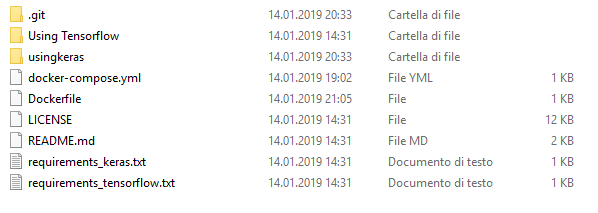
\includegraphics[width=1\textwidth]{Pictures/strutturaDirectory.PNG}
\end{figure}
\newline
E gestito correttamente alcuni dei suoi parametri: 
\begin{lstlisting}
Docker-compose.yml
version: '3'
services:
        keras:
                image: gnap/keras:latest
                volumes:
                        - ./usingkeras:/usingkeras
                entrypoint: /usingkeras/docker-entrypoint.sh
                stdin_open: true

\end{lstlisting}

\begin{lstlisting}
Dockerfile
FROM gw000/keras:2.1.4

RUN apt-get update -qq \
 && apt-get install --no-install-recommends -y \
    python-matplotlib \
    python-pillow
\end{lstlisting}

L'ambiente è pronto. Sarà quindi possibile inserire il dataset all'interno di questa struttura, nella cartella "usingkeras" per poi iniziare il training.

\subsubsection{Eseguire training e test del classificatore}
Per avviare il training del nostro classificatore di esempio, assicurarsi che il file "docker-entrypoint.sh" all'interno della cartella "usingkeras" sia impostato come segue:
\begin{lstlisting}
#!/bin/bash
cd /usingkeras/
python /usingkeras/Training.py 
#python /usingkeras/Testing.py
\end{lstlisting}

Successivamente, basta avviare il docker tramite il comando powershell:
\begin{lstlisting}
docker-compose up
\end{lstlisting}
Questo comando avvia il docker, esegue il contenuto del file "Docker-compose.yml" ed avvia lo script "/usingkeras/docker-entrypoint.sh"\Decaa
A questo punto basta aspettare il completamento del training, da notare che questa operazione richiede molta potenza di calcolo (occupazione della CPU) ed un po' di tempo, a dipendenza del numero di classi e delle epoche da fare:

\begin{figure}[h!]
  \centering
    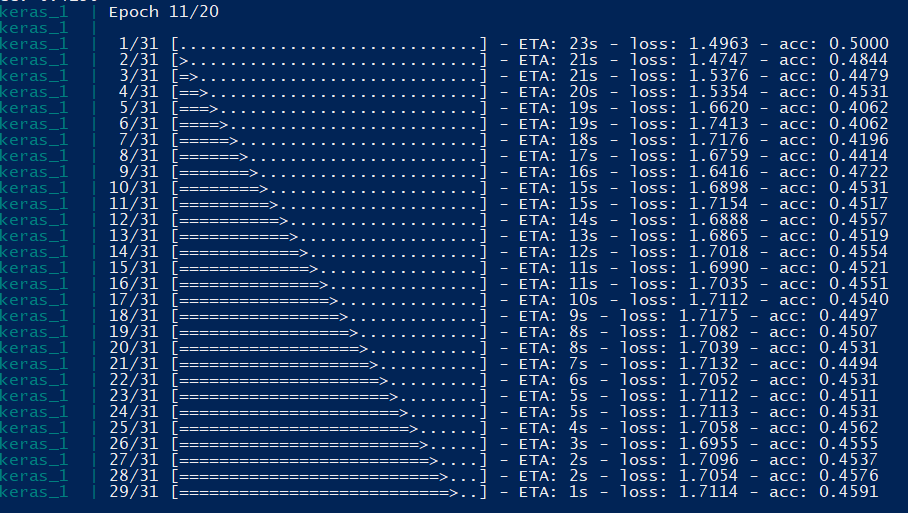
\includegraphics[width=1\textwidth]{Pictures/training.PNG}
\end{figure}
\newline

Al termine di questa operazione, il nostro classificatore con rete neurale è pronto.

\subsection{Test e risultati}%rob
I risultati ottenuti con TensorFlowSharp su desktop sono stati abbastanza buoni. I tempi di elaborazione rimangono tra i 100 e i 150 ms. L'accuratezza del classificatore non è ottimale, ritorna risultati intorno al 50-60\% quando riconosce un monitor. Dato che nel modello pre-addestrato erano presenti più di mille label, abbiamo aggiunto il metodo isMonitorOrSimilarLabel per includere anche i nomi di elementi simili come schermo o televisione, aumentandone la precisione. A livello mobile tuttavia non siamo riusciti a testare questa funzionalità per questioni tempistiche.
\Decaa
Il classificatore personalizzato creato per rilevare i loghi
\chapter{Conclusioni}
\section{Risultati ottenuti}
\subsection{Obbiettivi raggiunti}
Il primo obiettivo, quello di ritornare un'informazione associata data una fotografia è stato raggiunto. Infatti durante i nostri test il programma restituisce la stringa associata al momento della creazione della repository. 
Il secondo obiettivo era quello di sviluppare le funzionalità come una libreria, in modo che la ditta DSwiss potesse utilizzarla successivamente. Questo intento è stato raggiunto parzialmente. La libreria infatti è completamente fruibile a livello desktop per ciò che riguarda le funzioni di feature matching e di utilizzo di tecnologie di Machine Learning. Tuttavia la implementazione per dispositivi mobili non è stata testata per iOS e per la versione Android manca l'implementazione della funzione di ricerca monitor, cioé quella sviluppata per mostrare un possibile utilizzo delle tecnologie di apprendimento automatico.
Il terzo obiettivo è stato raggiunto pienamente in quanto tutto ciò che è stato sviluppato non richiede chiamate a codice esterno e tutte le operazioni sono elaborate localmente.
\subsection{Obbiettivi non raggiunti}
\section{Sviluppi futuri}%rob%rob
Per l'utilizzo della libreria su mobile abbiamo pensato ad un flusso di lavoro come questo:
\Decaa
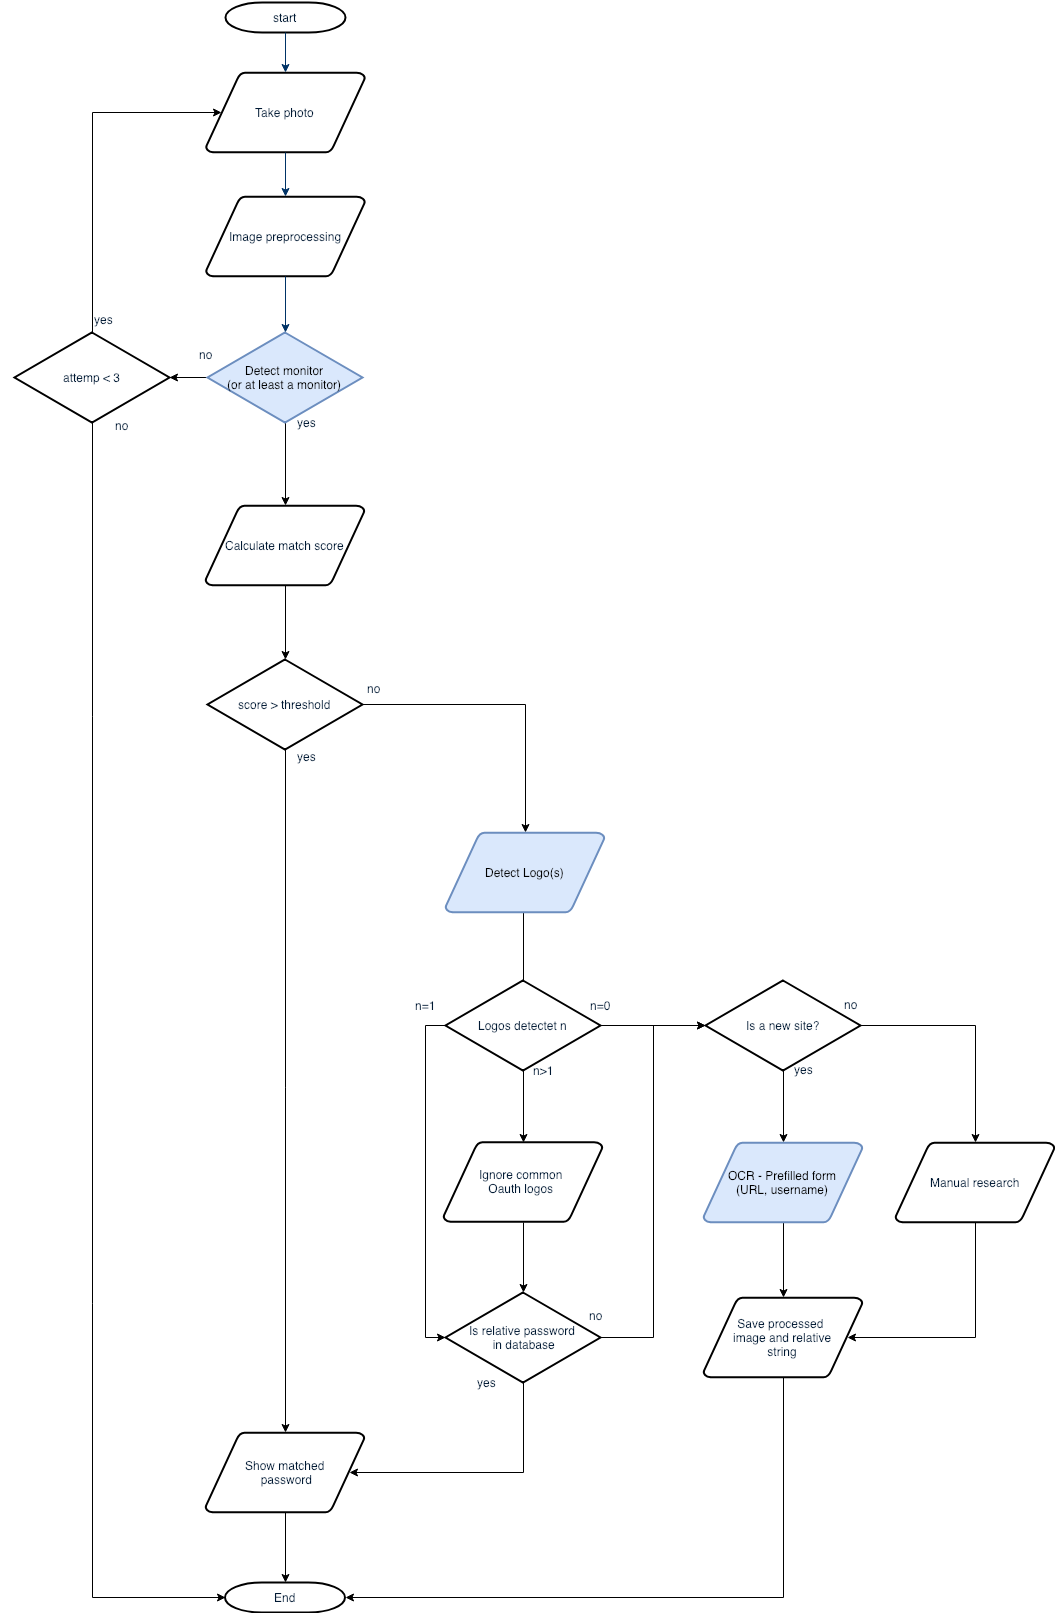
\includegraphics[width=\textwidth]{Pictures/flusso2.png}
\Decaa
%%%%%TODO%%%%
Gli elementi che sono ancora da implementare sono il riconoscimento del logo, una ottimizzazione della gestione della repository locale e l'implementazione di tecnologie OCR per favorire l'inserimento di nuovi dati da parte dell'utente.

\section{Competenze acquisite}%rob%rob
Grazie a questo lavoro abbiamo approfondito le nostre conoscenze in ambito di machine learning e nello specifico dell'utilizzo delle convolutional neural network per costruire classificatori, utilizzando tecnologie quali Tensorflow e approfondendo leggermente le nostre competenze riguardo il linguaggio Python (che abbiamo usato per addestrare l'ultimo layer di una rete neurale). Grazie alla ricerca effettuata abbiamo capito che strumenti per utilizzare Machine Learning e Computer Vision con un tool multipiattaforma quale Xamarin, sono ancora immaturi. Pertanto il nostro suggerimento è quello di affidarsi allo sviluppo nativo ma anche quello di valutare attentamente di non utilizzare risorse locali ma di delegare il compito a servizi esterni. 
\Decaa
Durante lo sviluppo della libreria e dell'implementazione della demo, abbiamo avuto l'opportunità di imparare le basi dell'utilizzo del framework Xamarin. 

\chapter{Piano dei lavori}%rob%rob
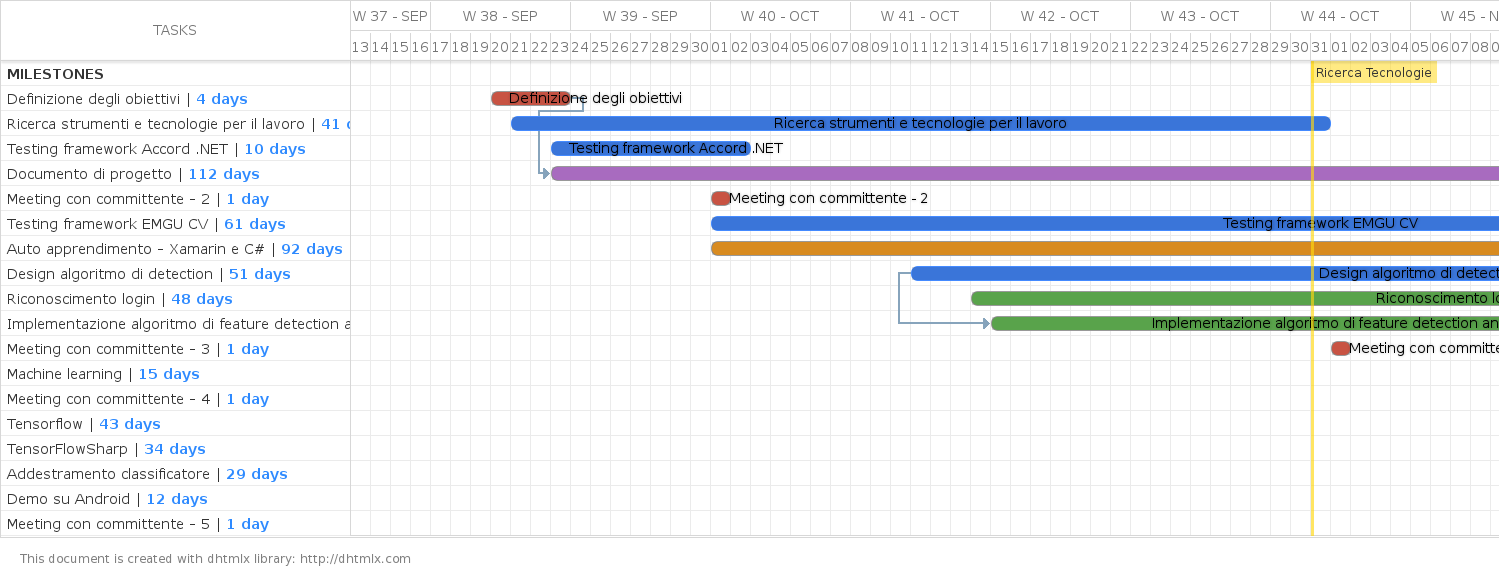
\includegraphics[width=\textwidth]{Pictures/Piano_lavori1.png}
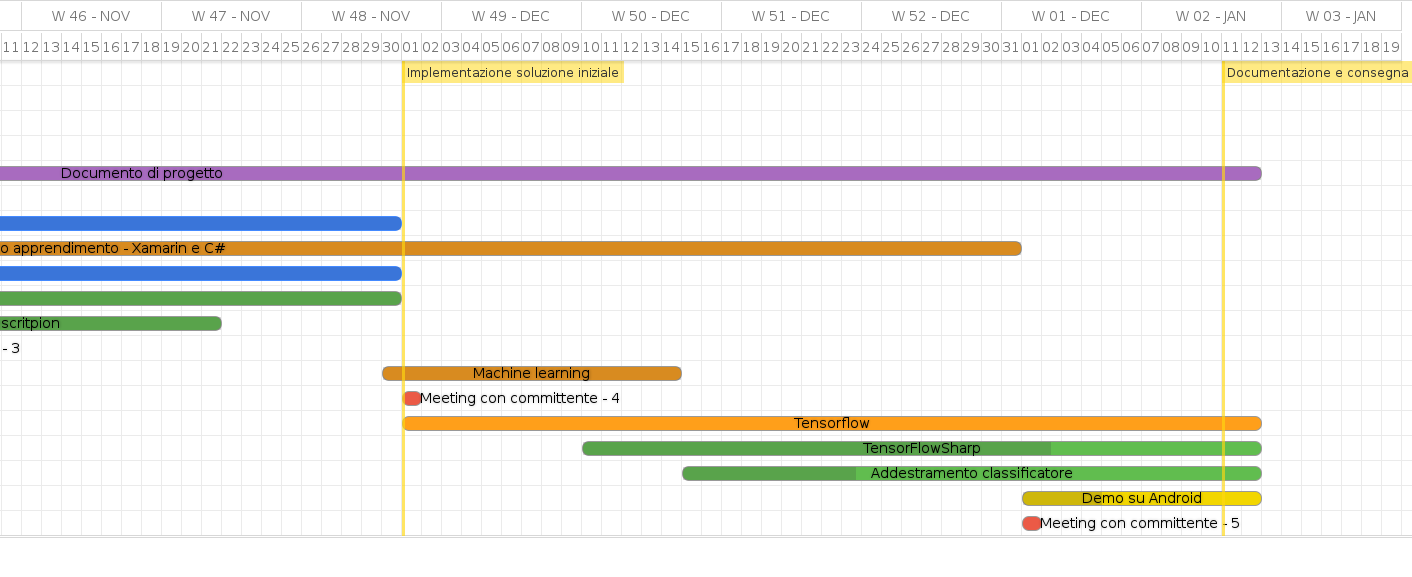
\includegraphics[width=\textwidth]{Pictures/Piano_lavori2.png}


%%% appendice %%%
% problemi riscontrati
% installazione ambienti di sviluppo
% installazione frameworks




%-------------------- Esempi da togliere -----------------------------------
% \chapter{Titolazione}

% \lipsum[13]

% \section{Sezione}

% \lipsum[23]
% Esempio di citazione \cite{4538384}, \cite{5357331,4523385}, \cite{1705631}.
% \footnote{Questa \`e una nota a pi\'e di pagina.}
% \footnote{Questa \`e un'altra nota a pi\'e di pagina.}
% \lipsum[23]

% \subsection{Sotto sezione}

% \texttt{Questo testo ha una spaziatura fissa}

% \textit{Questo testo \`e in italico}

% \textbf{Questo testo \`e in grassetto}

% \textsc{Questo testo \`e in maiuscoletto}

% \underline{Questo testo \`e sottolineato} \\

% Citazione:
% \begin{quote}
% \lipsum[23]
% \end{quote}

% \chapter{Titolazione}

% \lipsum[13]

% \begin{itemize}
%   \item Elemento A
%   \item Elemento B
%   \item Elemento C
% \end{itemize}

% %\begin{itemize}
% %  \item[-] Elemento A
% %  \item[-] Elemento B
% %  \item[-] Elemento C
% %\end{itemize}
% %
% %\begin{enumerate}
% %  \item Alpha
% %  \item Beta
% %  \item Gamma
% %\end{enumerate}

% \lipsum[23]
% %\section{Sezione}
% %
% %\lipsum[23]
% %
% %\subsection{Sotto sezione}
% %
% %Un po' di matematica: \newline
% %
% %\begin{math}
% %\frac{n!}{k!(n-k)!} = {n \choose k}
% %\end{math} \newline
% %
% %Un po' di matematica centrata:
% %
% %\begin{center}
% %\begin{math}
% %\frac{n!}{k!(n-k)!} = {n \choose k}
% %\end{math}
% %\end{center}
% %
% %Oppure con \$\$
% %
% %$$
% %\frac{n!}{k!(n-k)!} = {n \choose k}
% %$$
% %
% %Oppure anche direttamente nel testo ${1}\over{n}$ \\
% %
% %\lipsum[23]
\bibliographystyle{unsrt}
\bibliography{bibliografia}
\end{document}
